\section{Amodal-net Experiments}

We report quantitative results in~\tabref{tab:sailvos_quan}. 
%On the SAIL-VOS dataset, we 
% and compared with state-of-the-art method of~\cite{hu2019sail}. 
In the Amodal-net experiments, optical flow is used to align images in the history. All the results are reported using $T = 2$ frames. We also experimented with larger history. However, results did not change compared to using two frames. We suspect that usefulness of optical flow degrades as the history increases. %\as{don't forget to bold all columns}

As shown in \tabref{tab:sailvos_quan}, Amodal-net outperforms baselines~\cite{hu2019sail} by $3.5\%$ AP in the class-specific setting and by $3.6\%$ %{\bf\color{orange}3.6 is right?(40.8 to 43.8) 3.0?}\ray{That's AP50}
AP in the class-agnostic setting. We also observe gains on the other metrics except for $\text{AP}_{\text{50}}^{\text{H}}$ in the class-agnostic setting. These results validate that the proposed backbone and the box/mask-head tailored for amodal segmentation are effective and improve results.


We provide qualitative results in~\figref{fig:qual_result}. Note that our approach successfully predicts the amodal mask despite occlusions. 
In column 1, half of the person is occluded by a table. The model correctly infers the lower half of the person. In column 2, our approach correctly predicts the overlapping amodal boxes, inferring a car and a person.
In column 3, we successfully segment  the entire motorcycle, propagating information `through' the person.
In column 4, the segmentations of the laptop and person correctly maintain their corresponding boundaries.   
%In contrast, the baseline suffers from duplicate detections, \eg, the second column, and challenges with the amodal segmentation. 
%For example, 
%In column three, the motorcycle is not fully segmented, or in column four, where the segmentation of the laptop and person mixes. 
%\as{make this paragraph stronger; relate it back to the three issues explained in the intro; don't emphasize what goes wrong in prior work but what our method does better; don't trash others, emphasize ours} %\as{order columns (left to right) to match discussion}



Next, we conduct an ablation study to assess the merits of the proposed components.  \tabref{tab:ablation} shows that each of the proposed components leads to improvements in the amodal mask's AP.
In row 2, we validated that multi-task training with occlusion annotations is beneficial. 
%In row 2, we observe that using and additional occlusion branch is beneficial. 
To experiment with different numbers of mask layers, we freeze the box-branch and only train the amodal mask.
In row 3 and 4, we observe that using nine mask layers achieves the best results and adding more layers doesn't improve further. In row 5, we validated that the use of flow is effective. 
In row 6 and 7, we see that the cascade box regression along with Soft-NMS leads to improvements in box AP. Lastly, in row 8, further refinement with mask iterations also improves the amodal segmentation's accuracy.
%!TEX root = main.tex

\begin{figure*}[t]
    \centering
    \setlength{\tabcolsep}{1pt}
    %\renewcommand{\arraystretch}{0.5}
    \renewcommand{\arraystretch}{4.3}
    \begin{tabular}{ccccc}
    % GT
    GT & 
    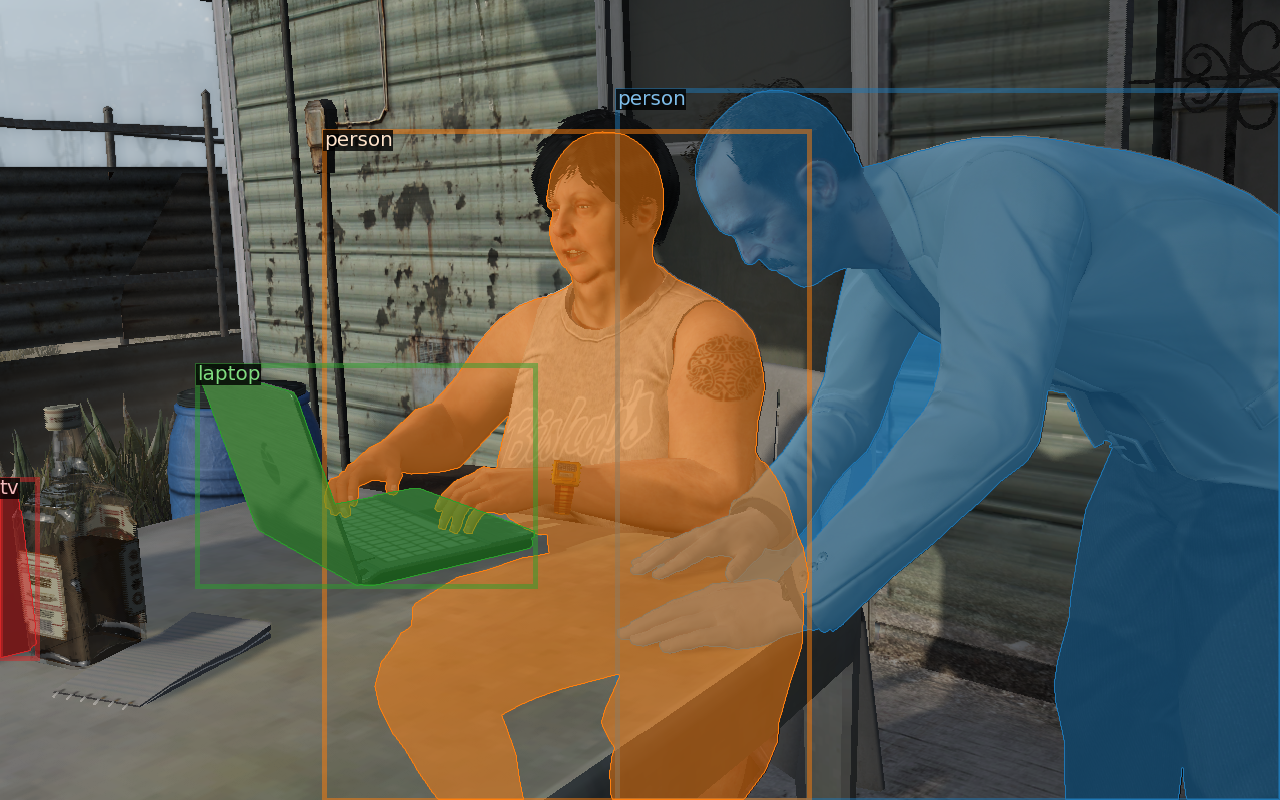
\includegraphics[align=c,width=0.23\linewidth]{fig/sailvos_results/21781_gt} &
    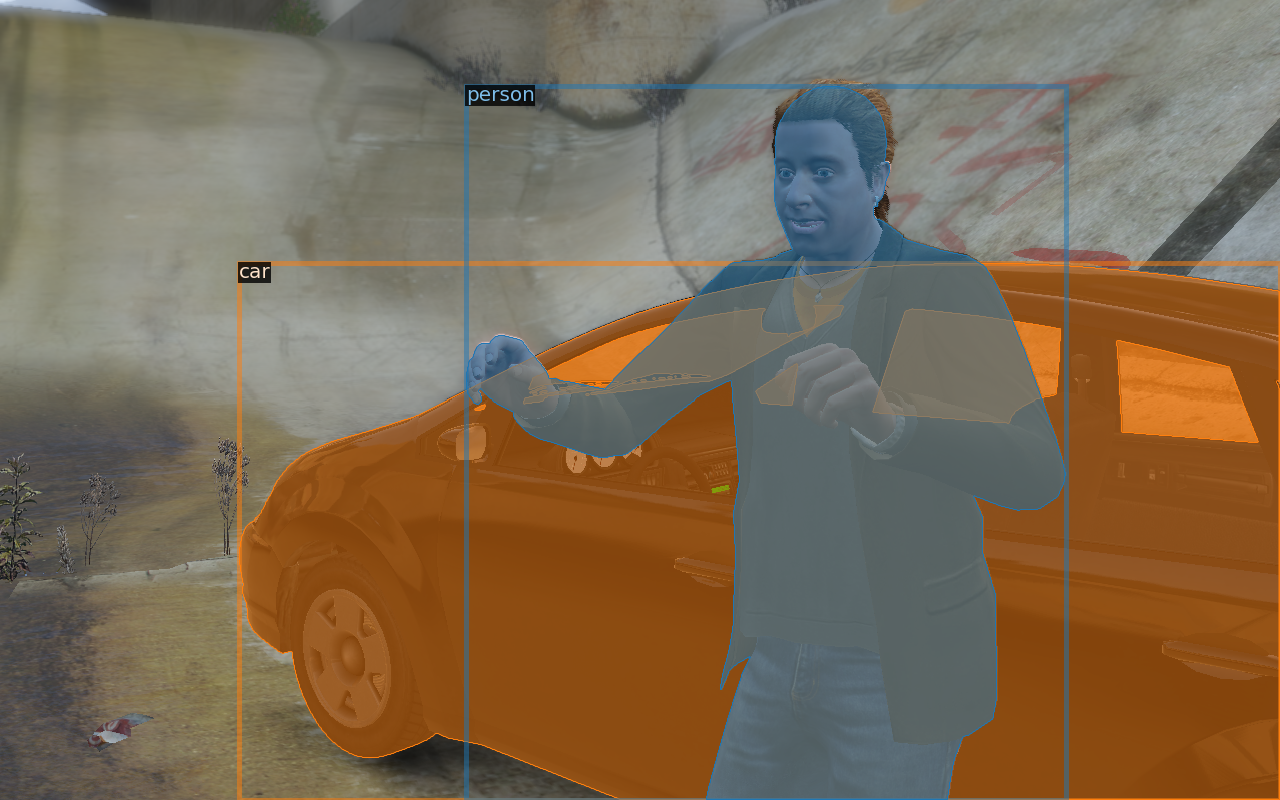
\includegraphics[align=c,width=0.23\linewidth]{fig/sailvos_results/10561_gt} &
    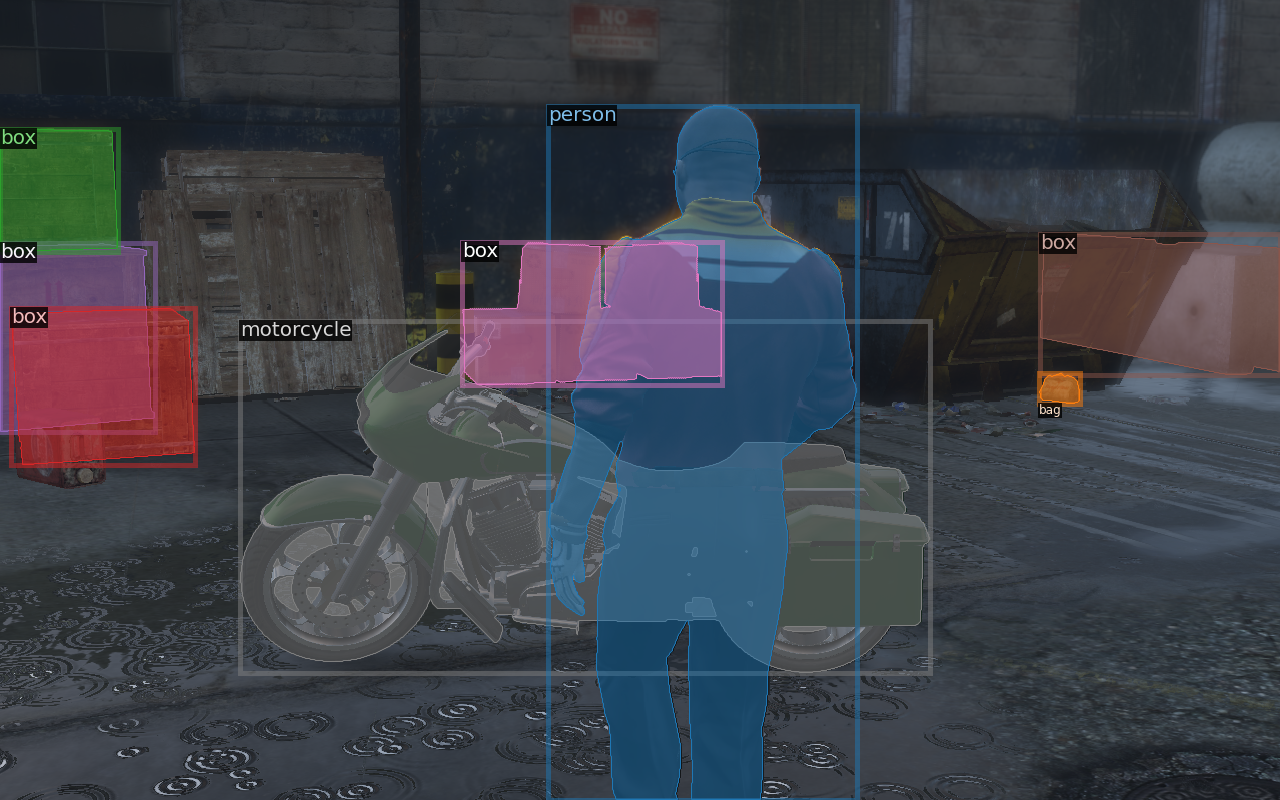
\includegraphics[align=c,width=0.23\linewidth]{fig/sailvos_results/14498_gt} &
    %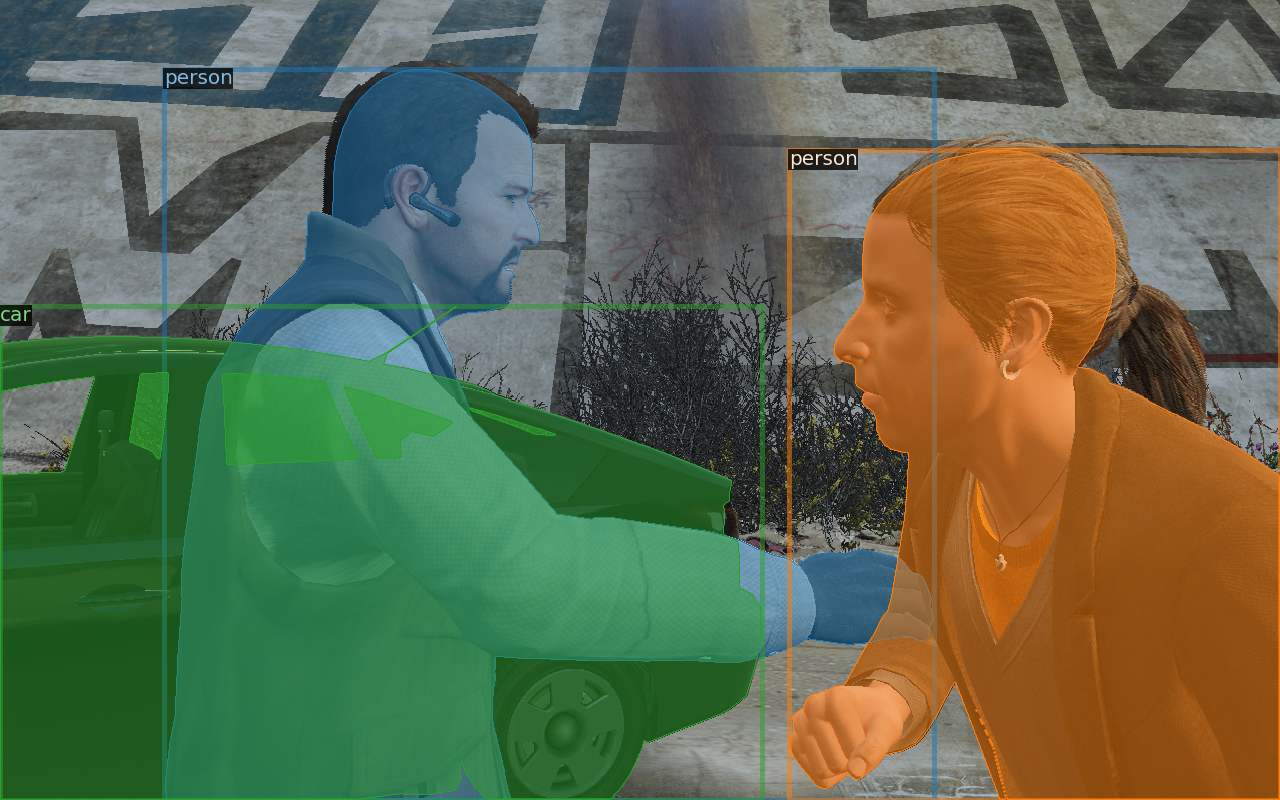
\includegraphics[align=c,width=0.23\linewidth]{fig/sailvos_results/11413_gt} &
    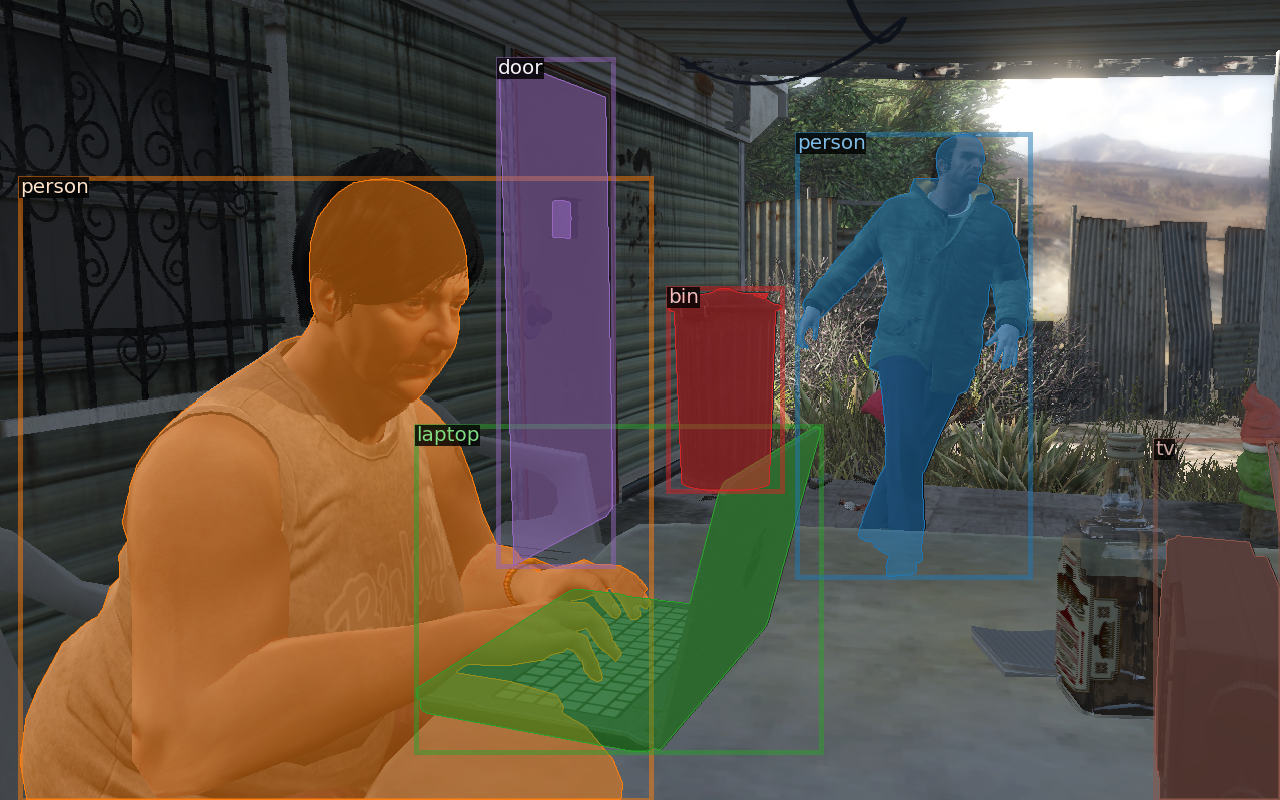
\includegraphics[align=c,width=0.23\linewidth]{fig/sailvos_results/22243_gt}
    \\
    % Baseline 
    \cite{hu2019sail} & 
    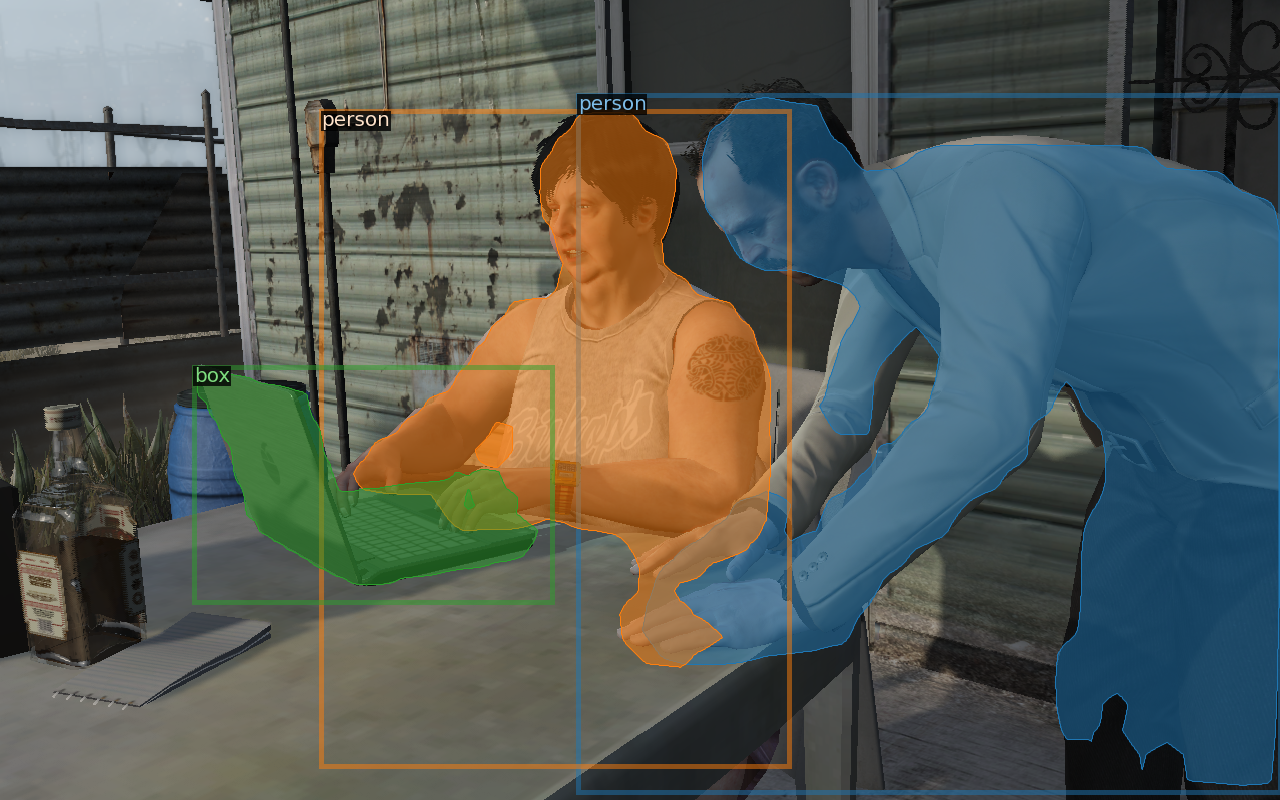
\includegraphics[align=c,width=0.23\linewidth]{fig/sailvos_results/21781_base} &
    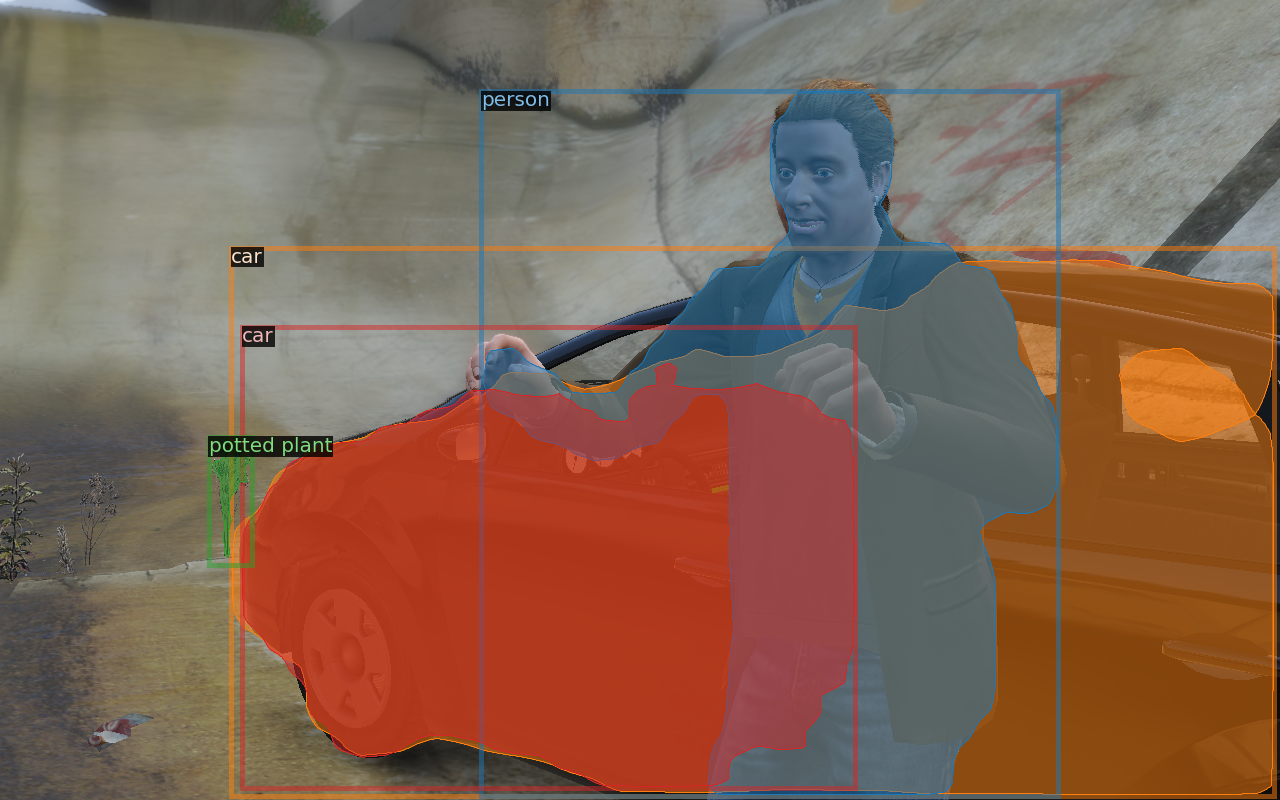
\includegraphics[align=c,width=0.23\linewidth]{fig/sailvos_results/10561_base} &
    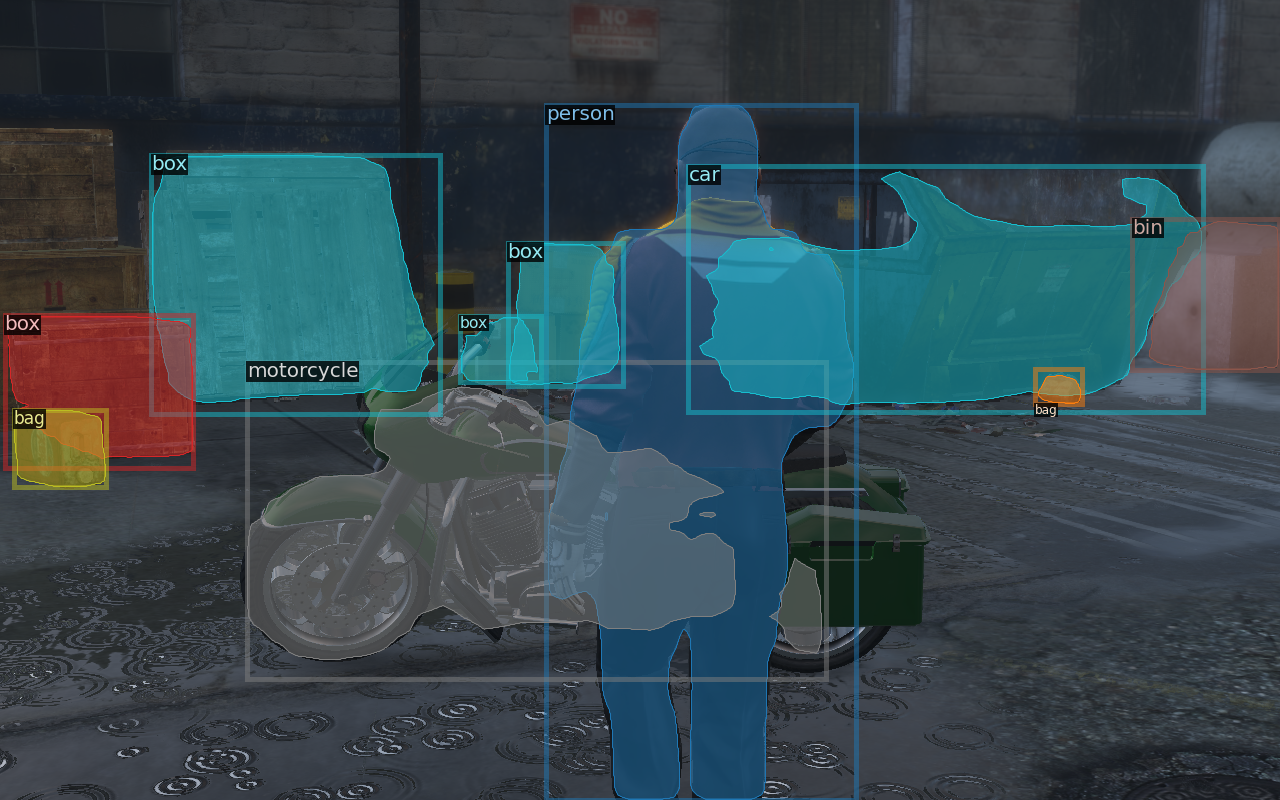
\includegraphics[align=c,width=0.23\linewidth]{fig/sailvos_results/14498_base} &
    %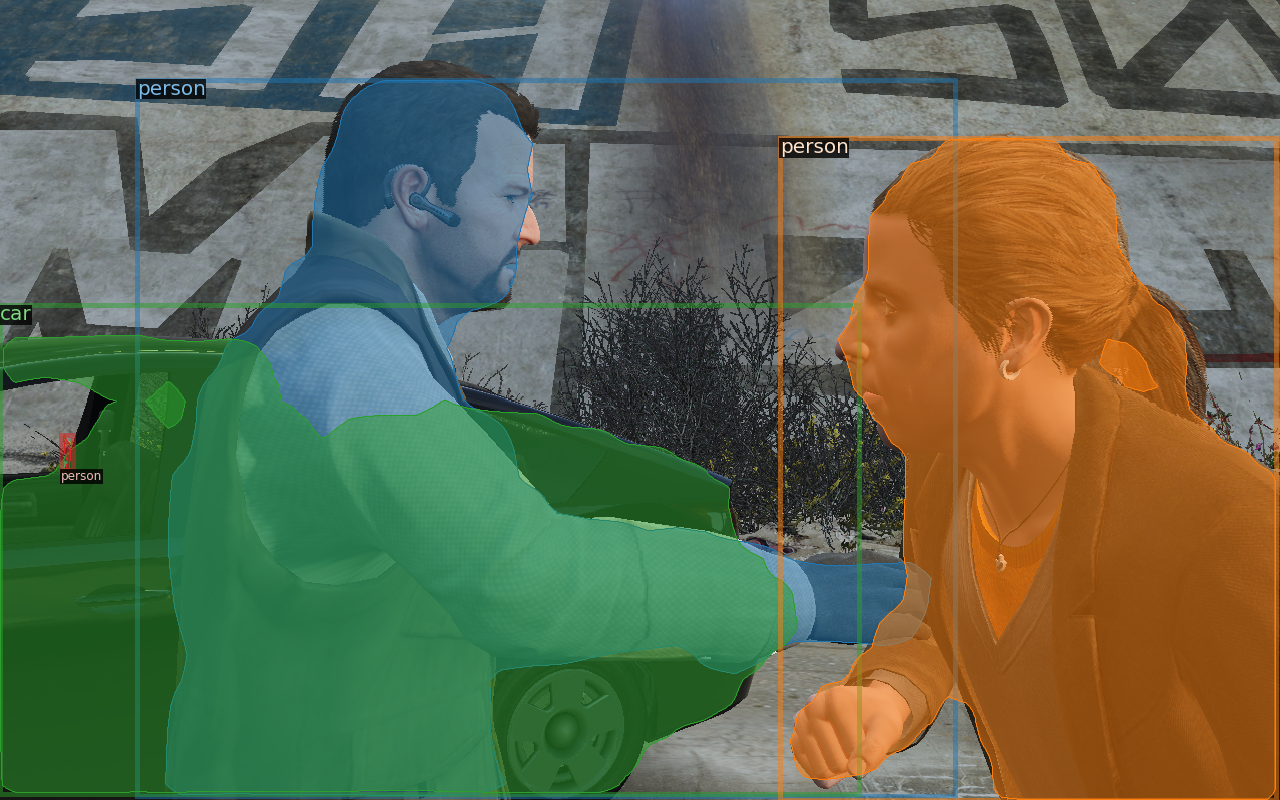
\includegraphics[align=c,width=0.23\linewidth]{fig/sailvos_results/11413_base} &
    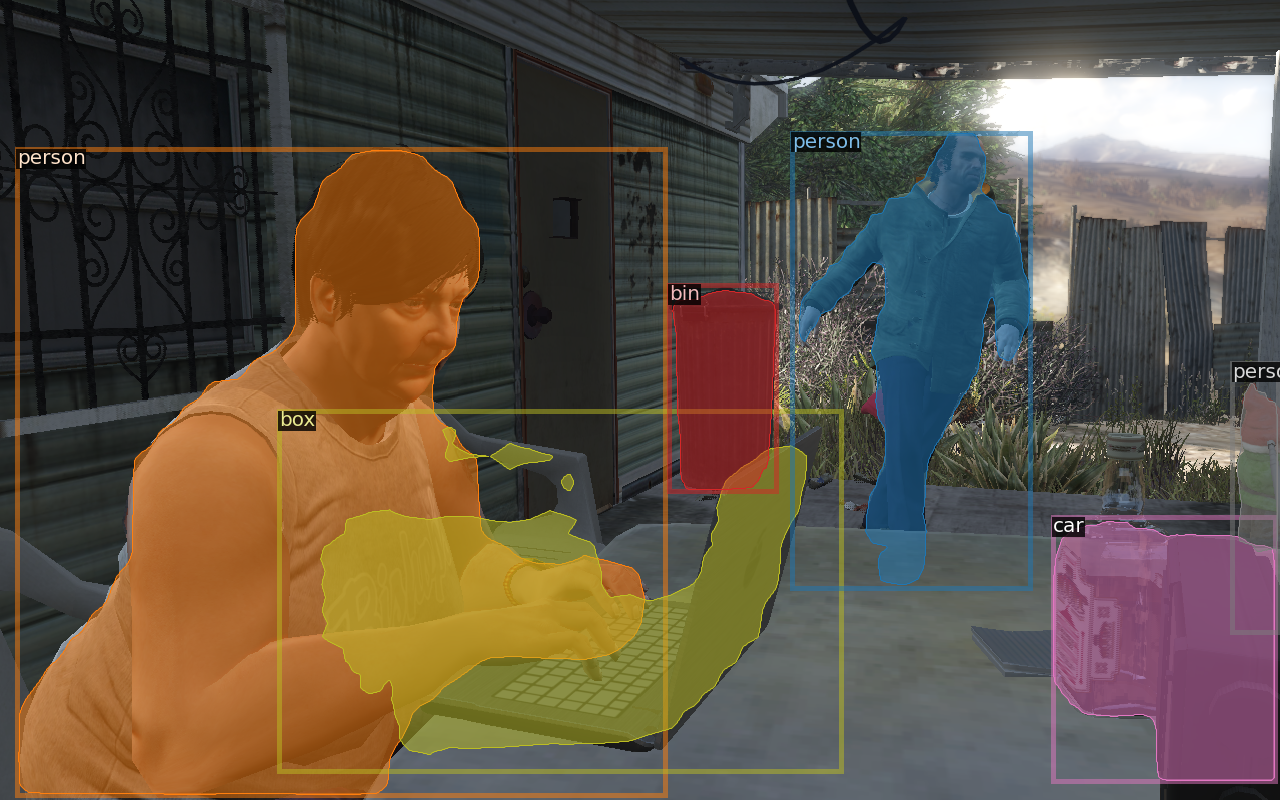
\includegraphics[align=c,width=0.23\linewidth]{fig/sailvos_results/22243_base}
    \\
    % Ours
    Ours &
    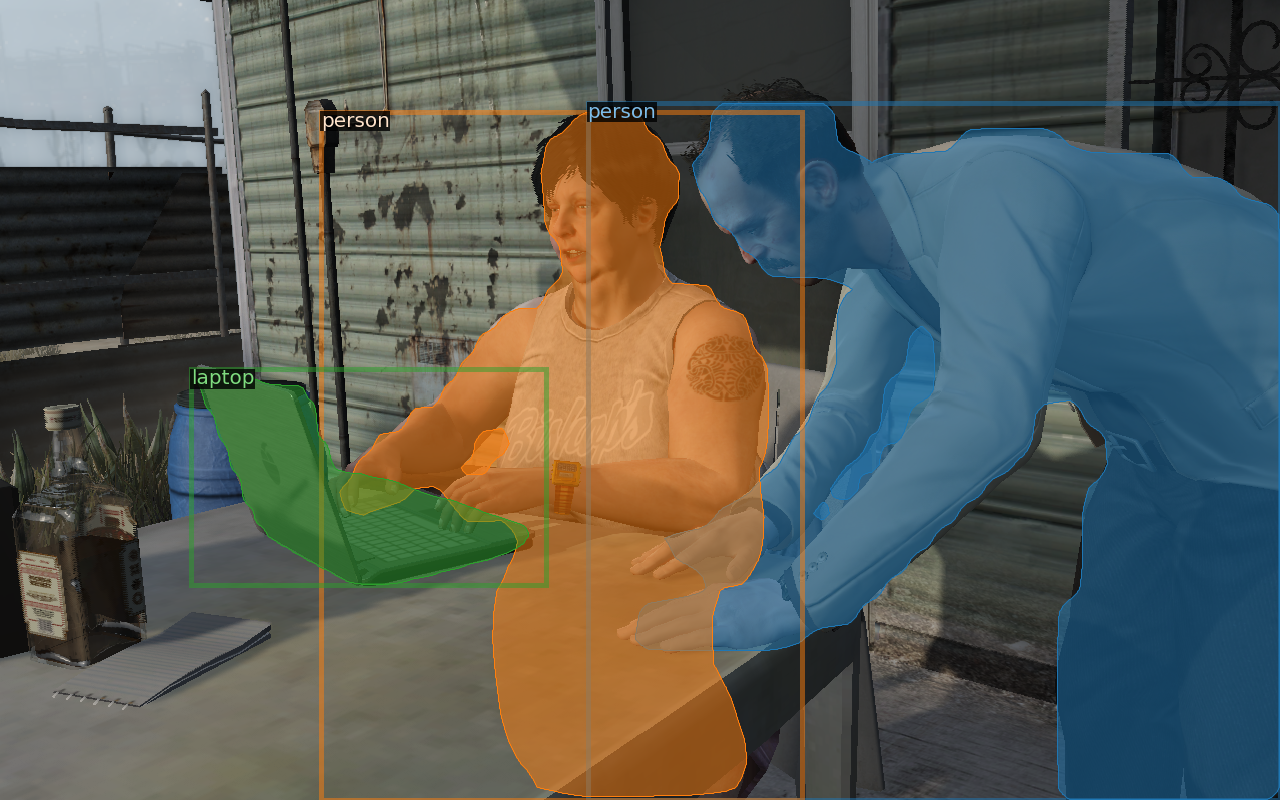
\includegraphics[align=c,width=0.23\linewidth]{fig/sailvos_results/21781_ours} &
    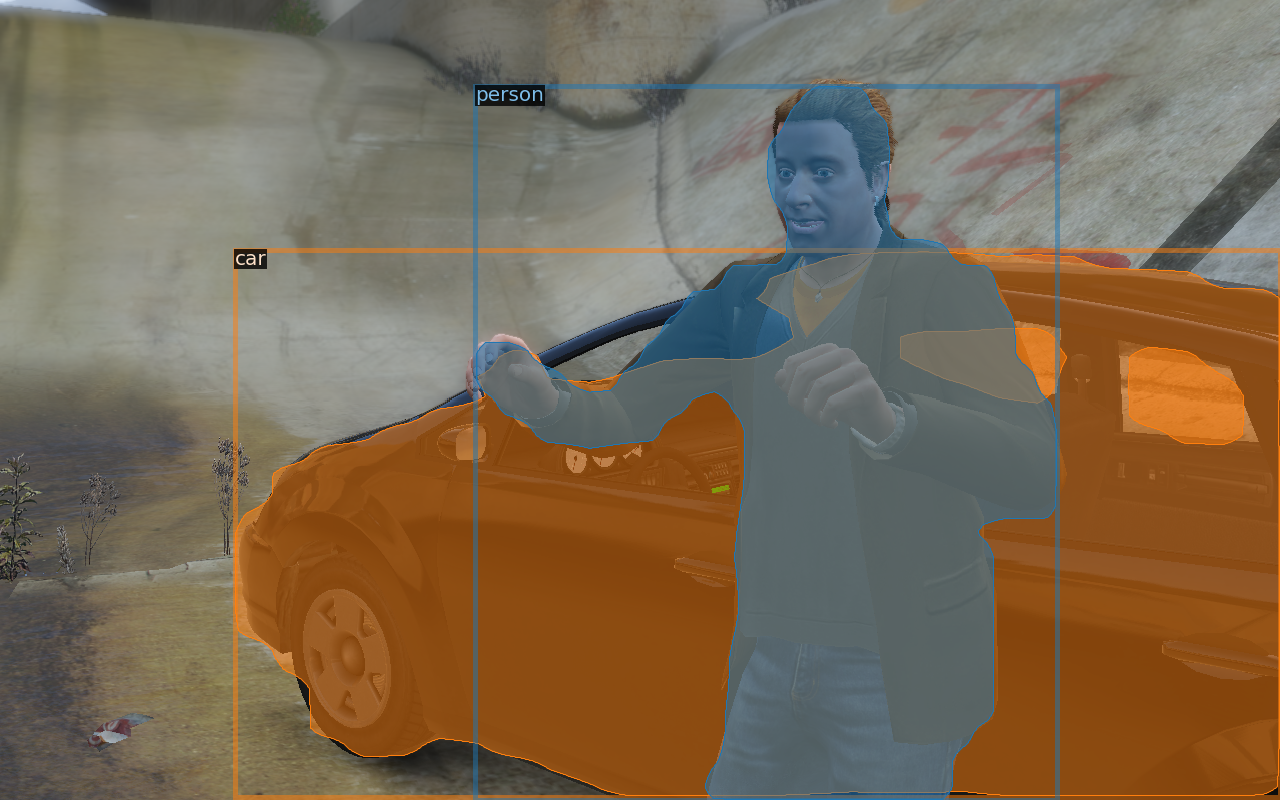
\includegraphics[align=c,width=0.23\linewidth]{fig/sailvos_results/10561_ours} &
    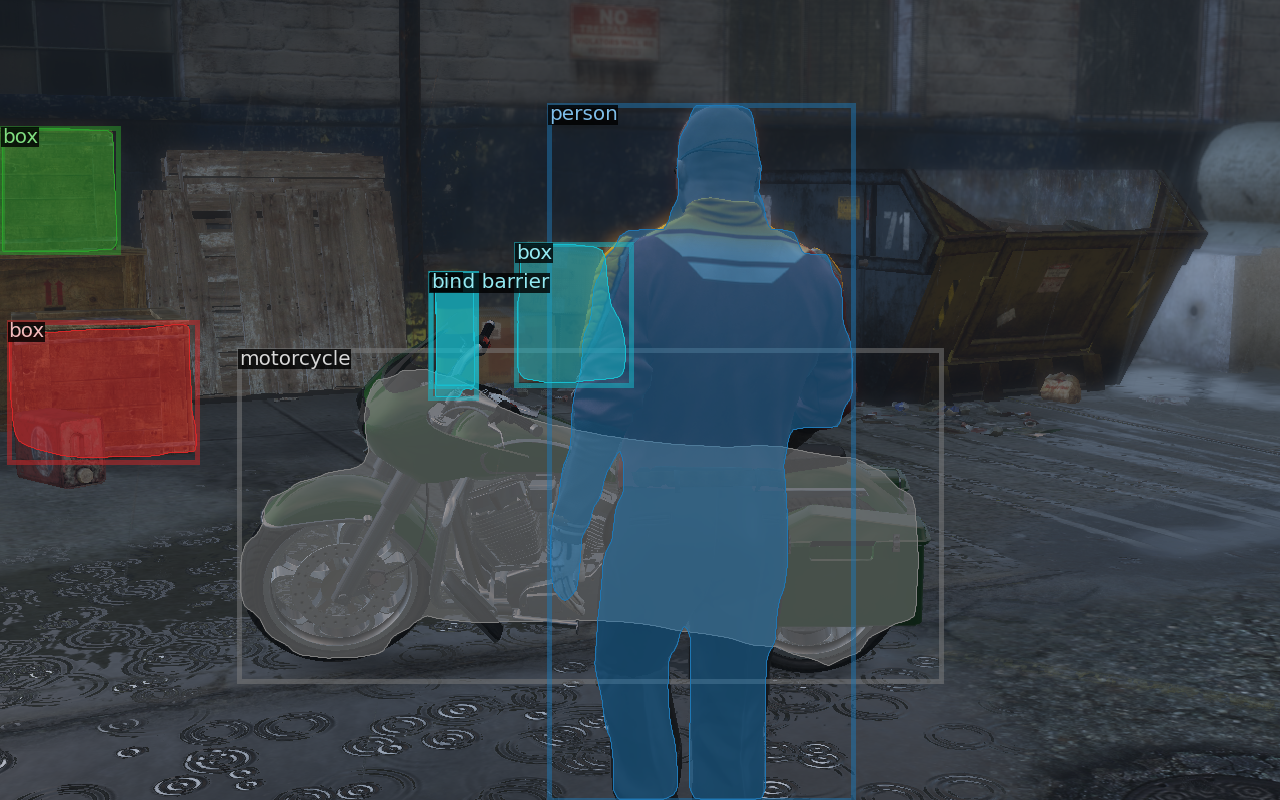
\includegraphics[align=c,width=0.23\linewidth]{fig/sailvos_results/14498_ours} &
    %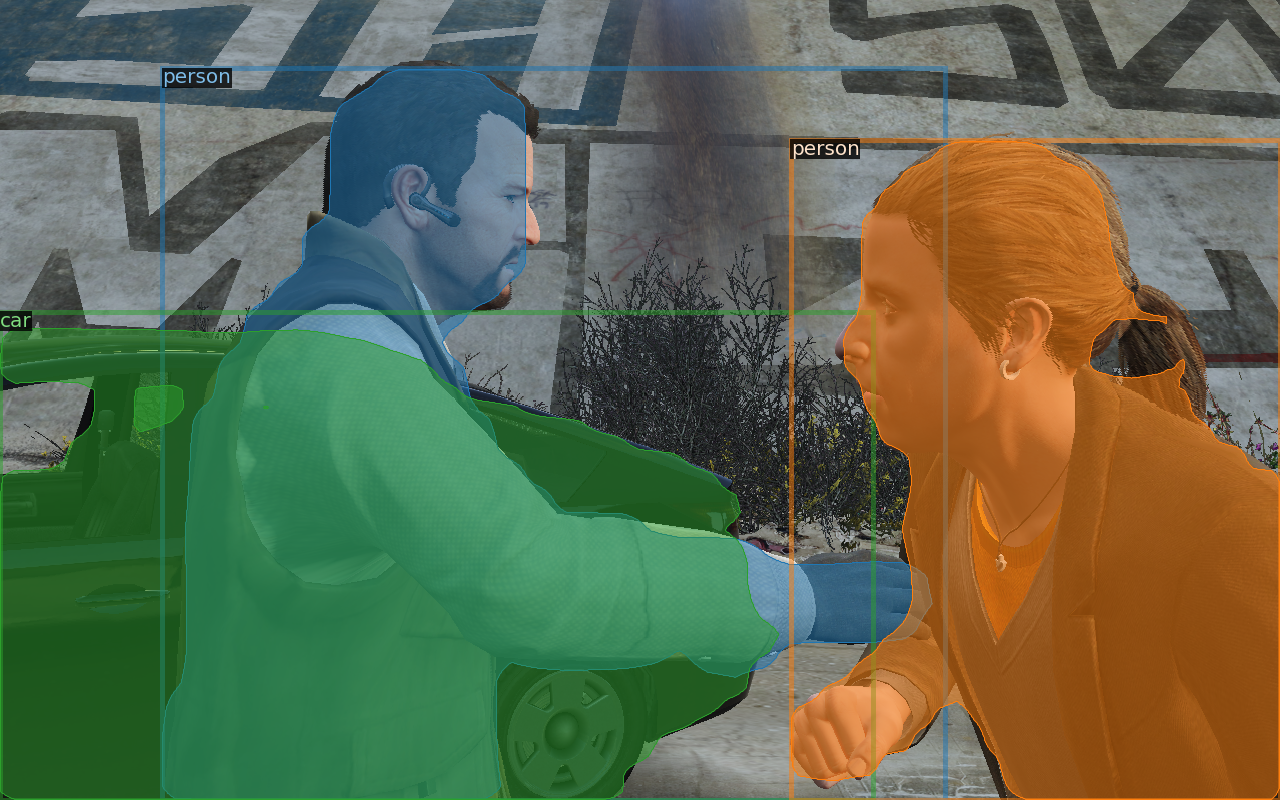
\includegraphics[align=c,width=0.23\linewidth]{fig/sailvos_results/11413_ours} &
    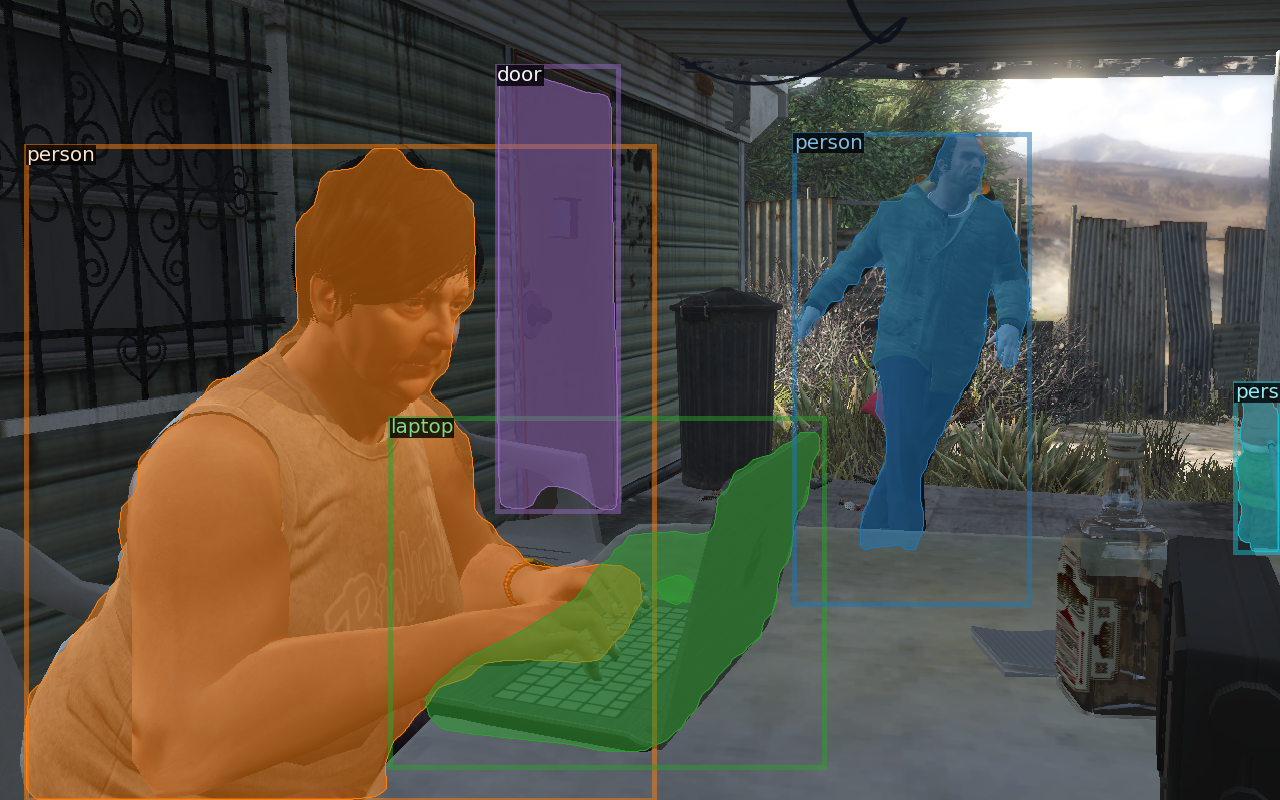
\includegraphics[align=c,width=0.23\linewidth]{fig/sailvos_results/22243_ours}
    \end{tabular}
    \vspace{-0.25cm}
    \caption{Qualitative comparison with~\cite{hu2019sail} on SAIL-VOS dataset in the class-specific setting.
    %\as{using the class-specific setting?}.
    }
    \label{fig:qual_result}
    \vspace{-0.25cm}
    \end{figure*}
    
    
    
    %\begin{tabular}{ccccc}
    %% GT
    %GT & 
    %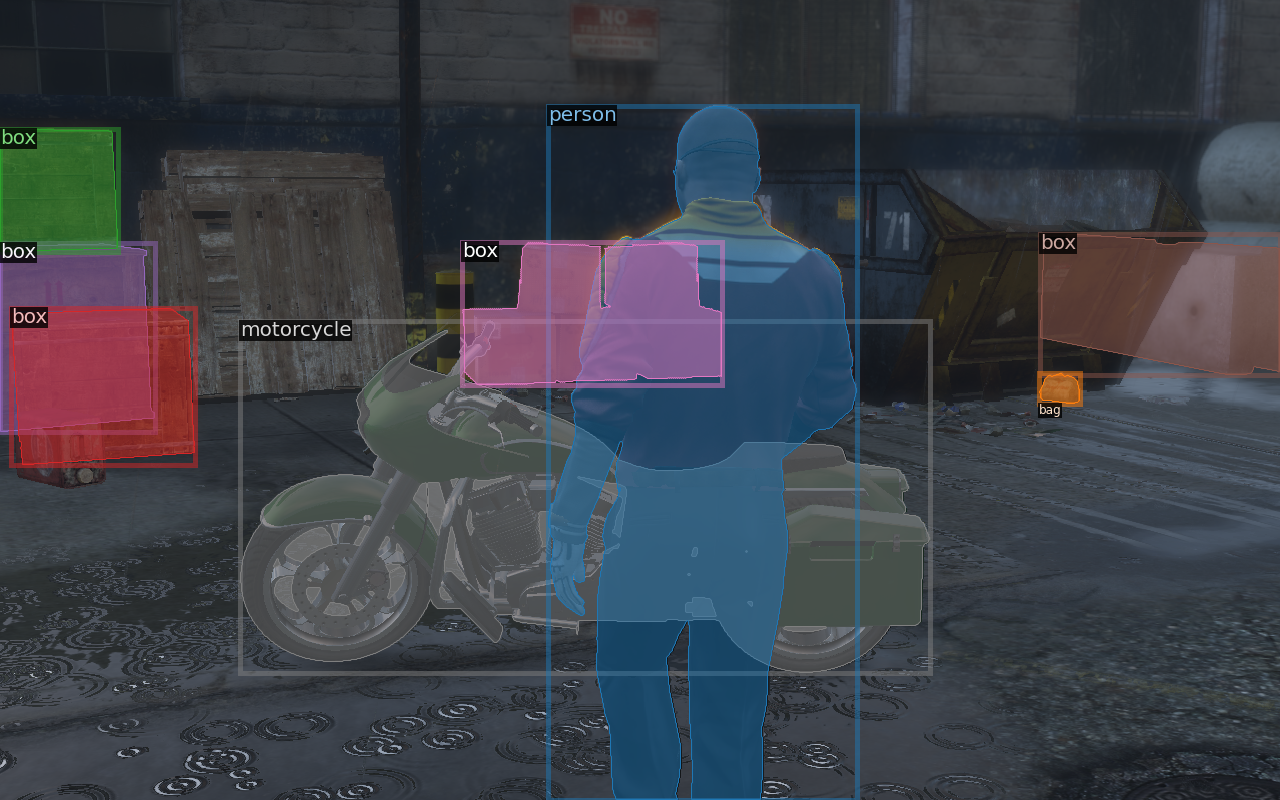
\includegraphics[align=c,width=0.23\linewidth]{fig/sailvos_results/14498_gt} &
    %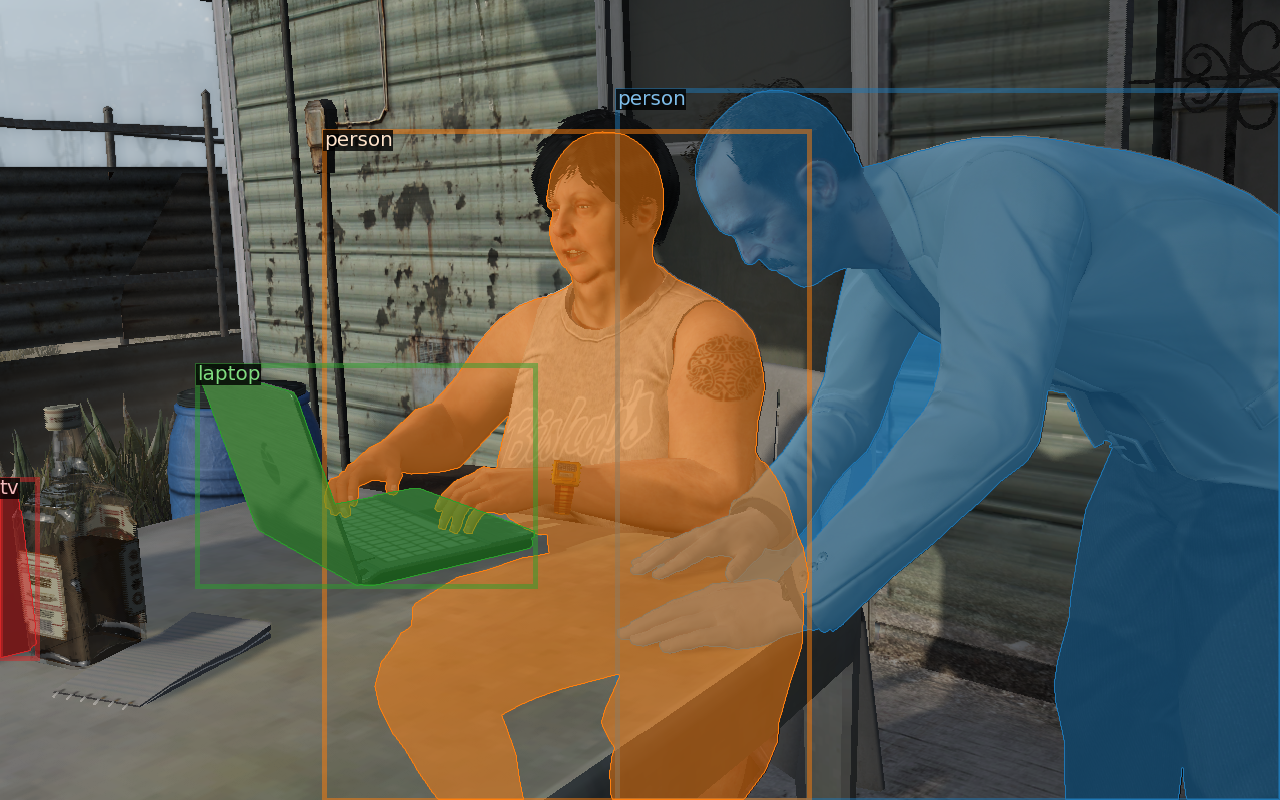
\includegraphics[align=c,width=0.23\linewidth]{fig/sailvos_results/21781_gt} &
    %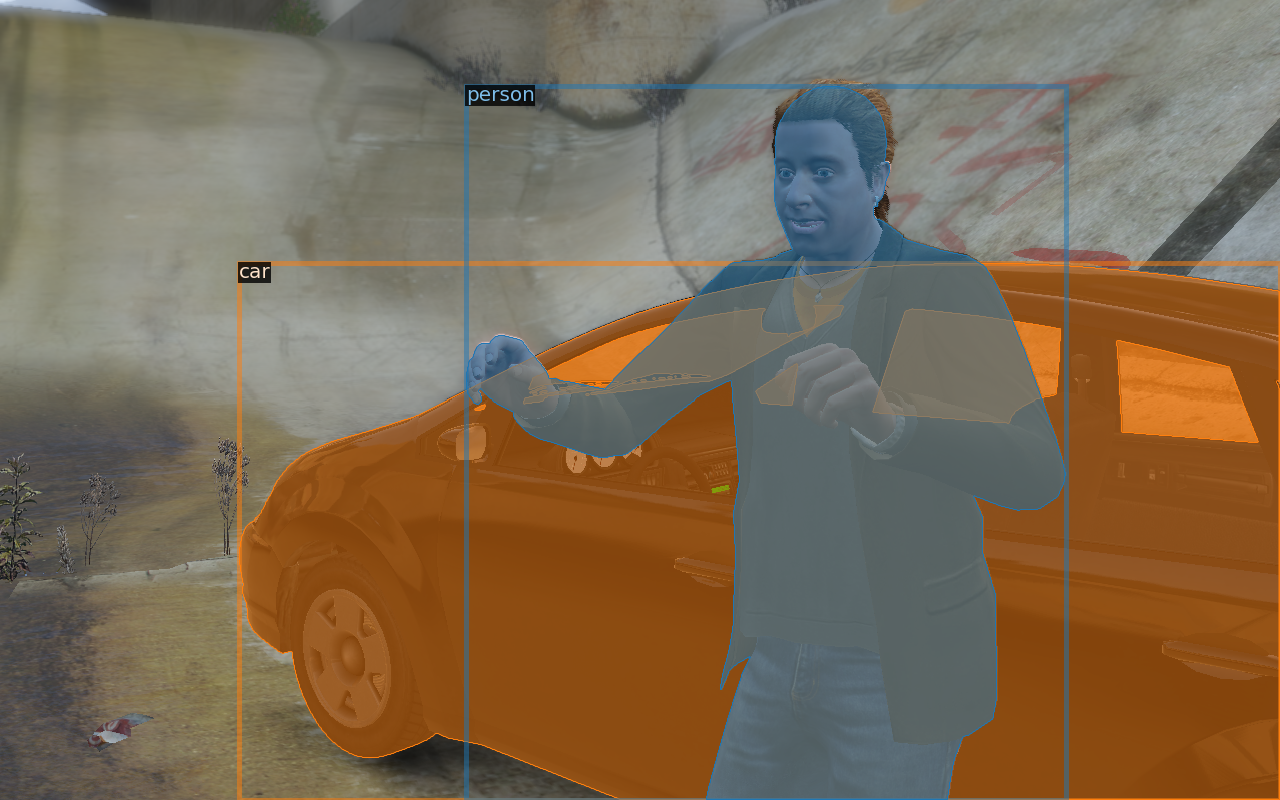
\includegraphics[align=c,width=0.23\linewidth]{fig/sailvos_results/10561_gt} &
    %%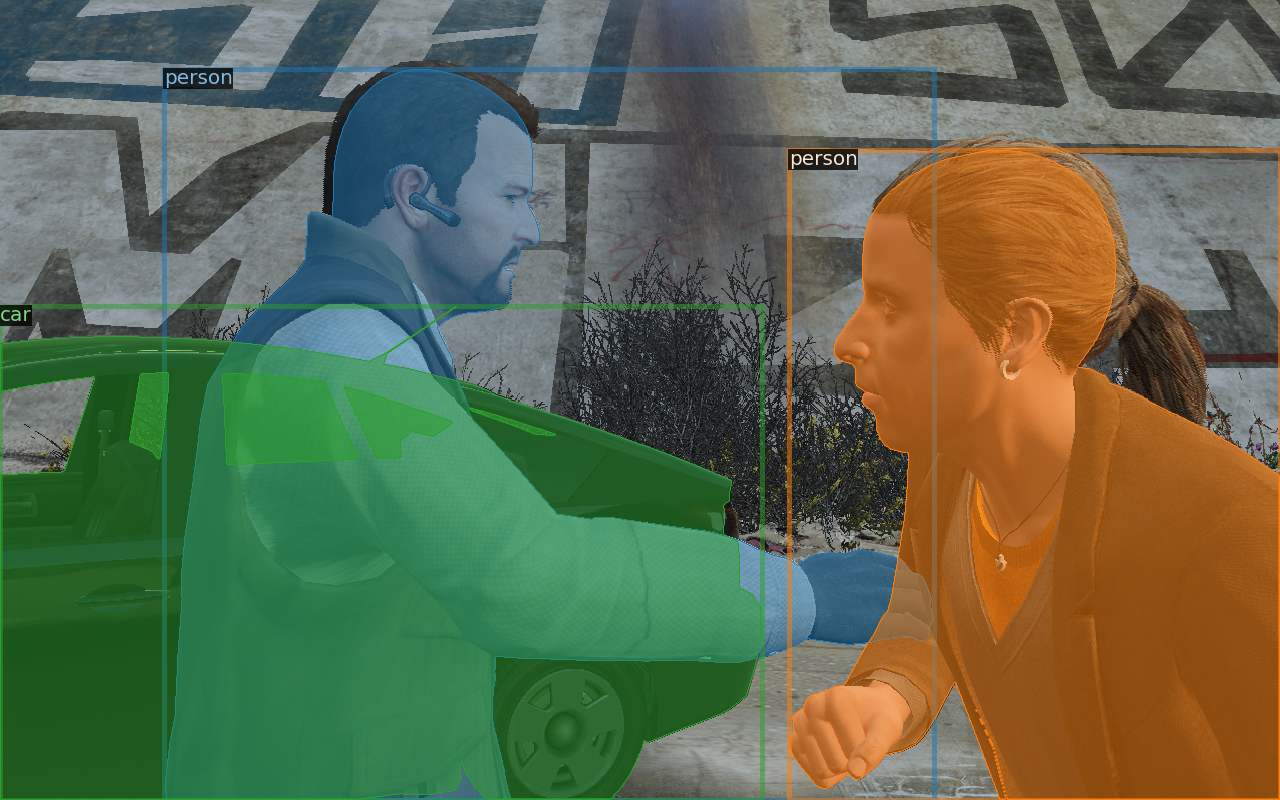
\includegraphics[align=c,width=0.23\linewidth]{fig/sailvos_results/11413_gt} &
    %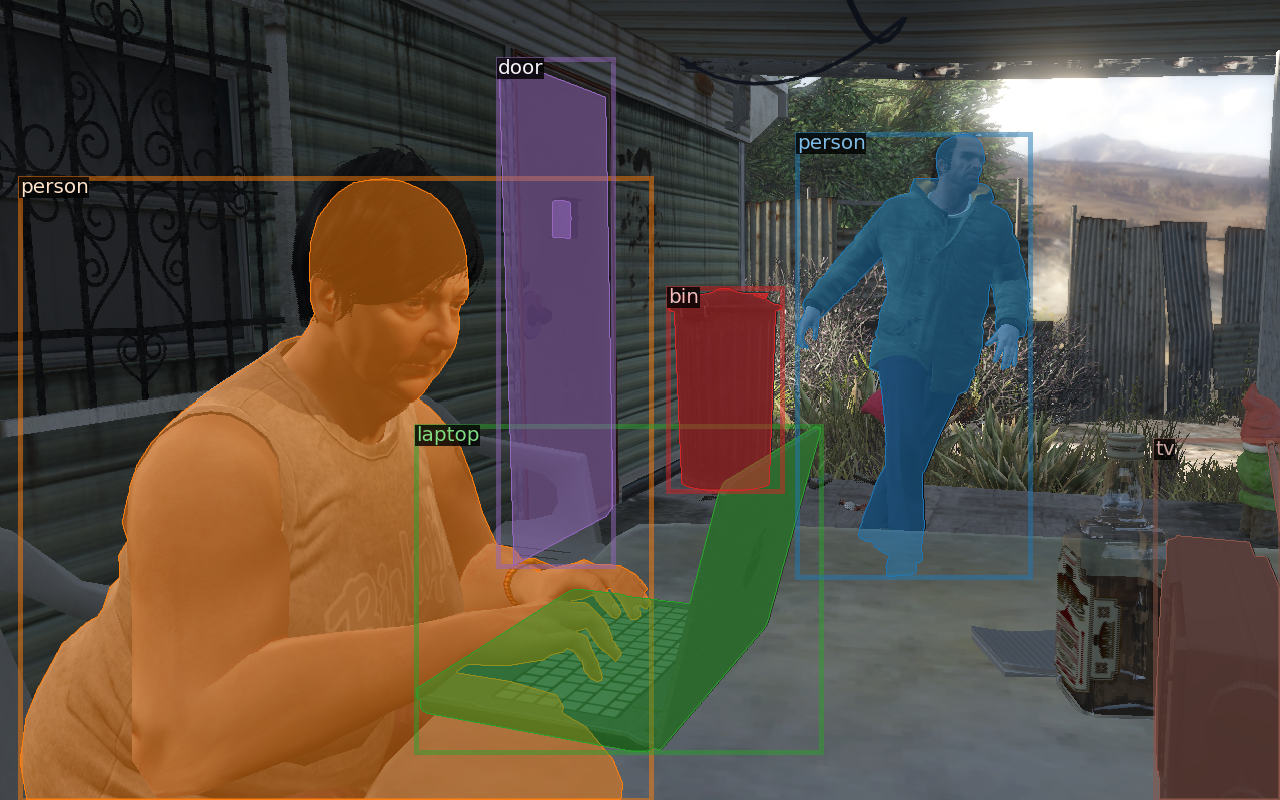
\includegraphics[align=c,width=0.23\linewidth]{fig/sailvos_results/22243_gt}
    %\\
    %% Baseline 
    %\cite{hu2019sail} & 
    %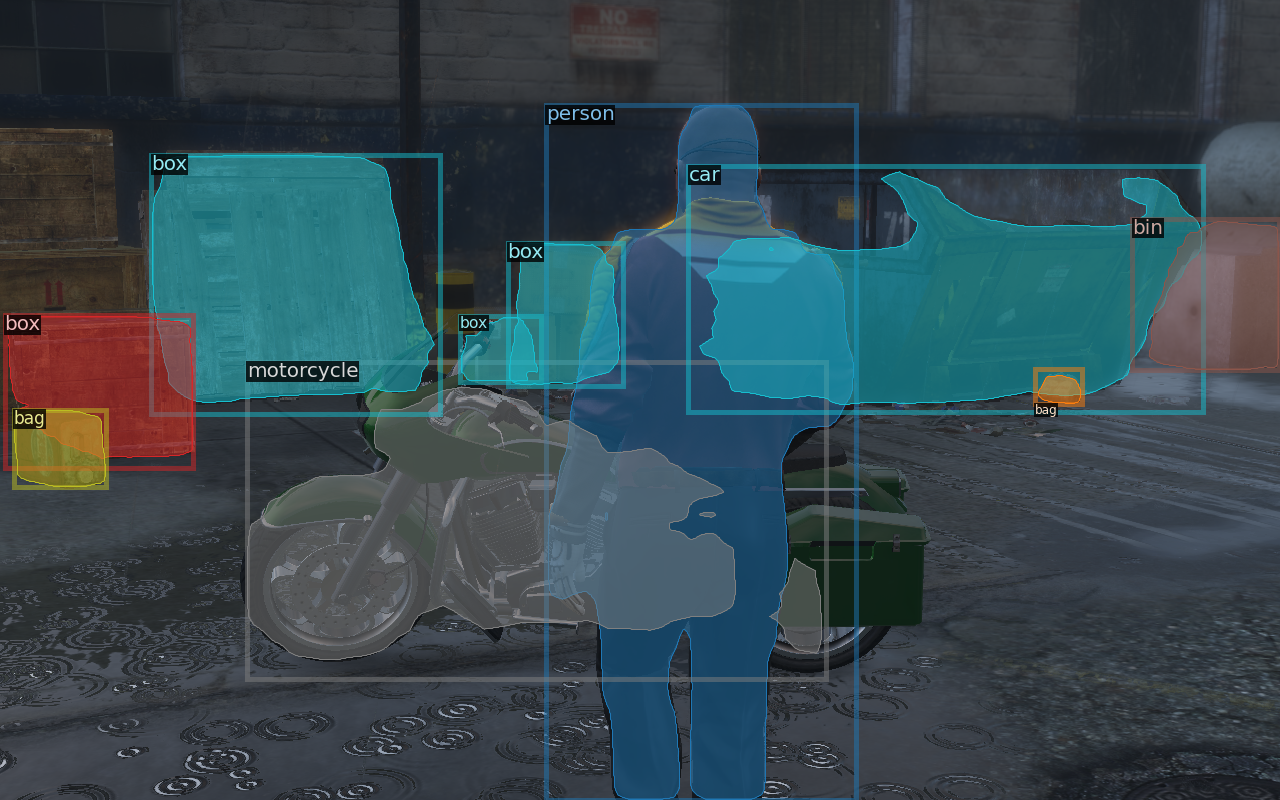
\includegraphics[align=c,width=0.23\linewidth]{fig/sailvos_results/14498_base} &
    %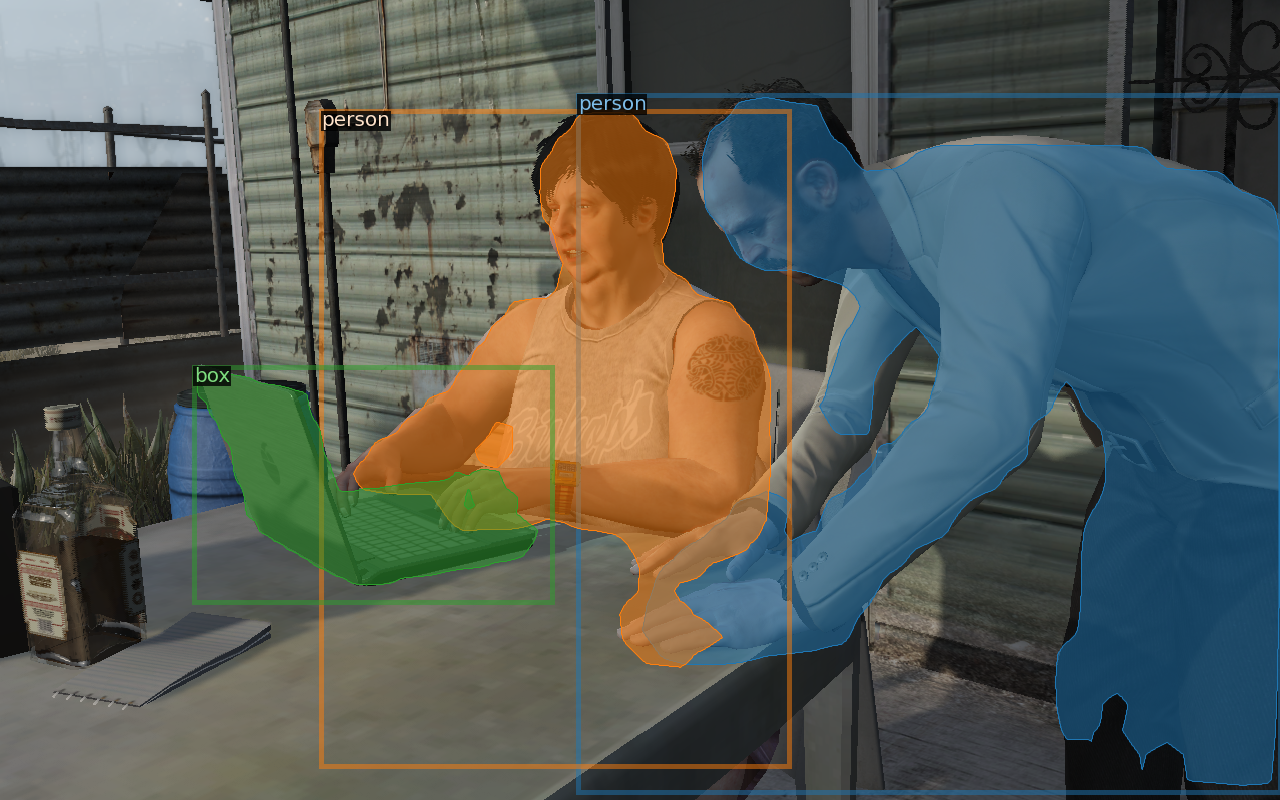
\includegraphics[align=c,width=0.23\linewidth]{fig/sailvos_results/21781_base} &
    %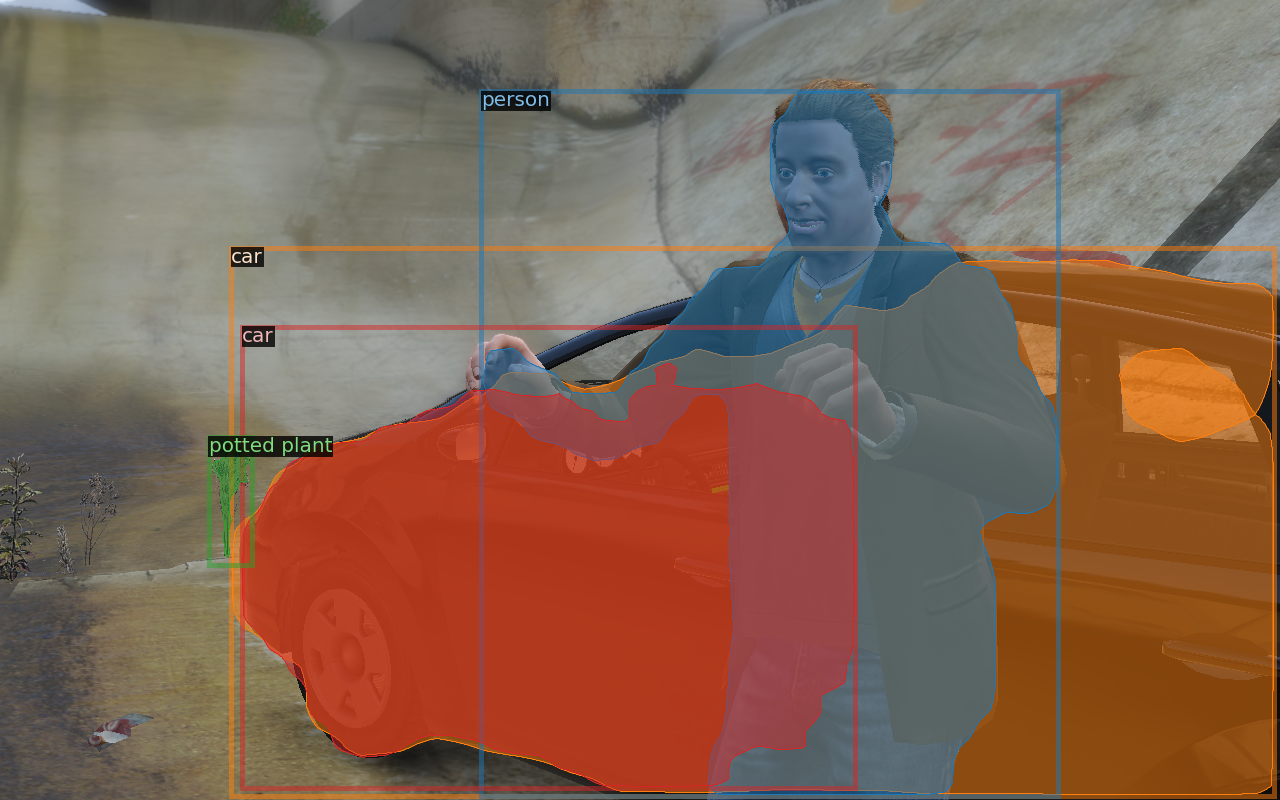
\includegraphics[align=c,width=0.23\linewidth]{fig/sailvos_results/10561_base} &
    %%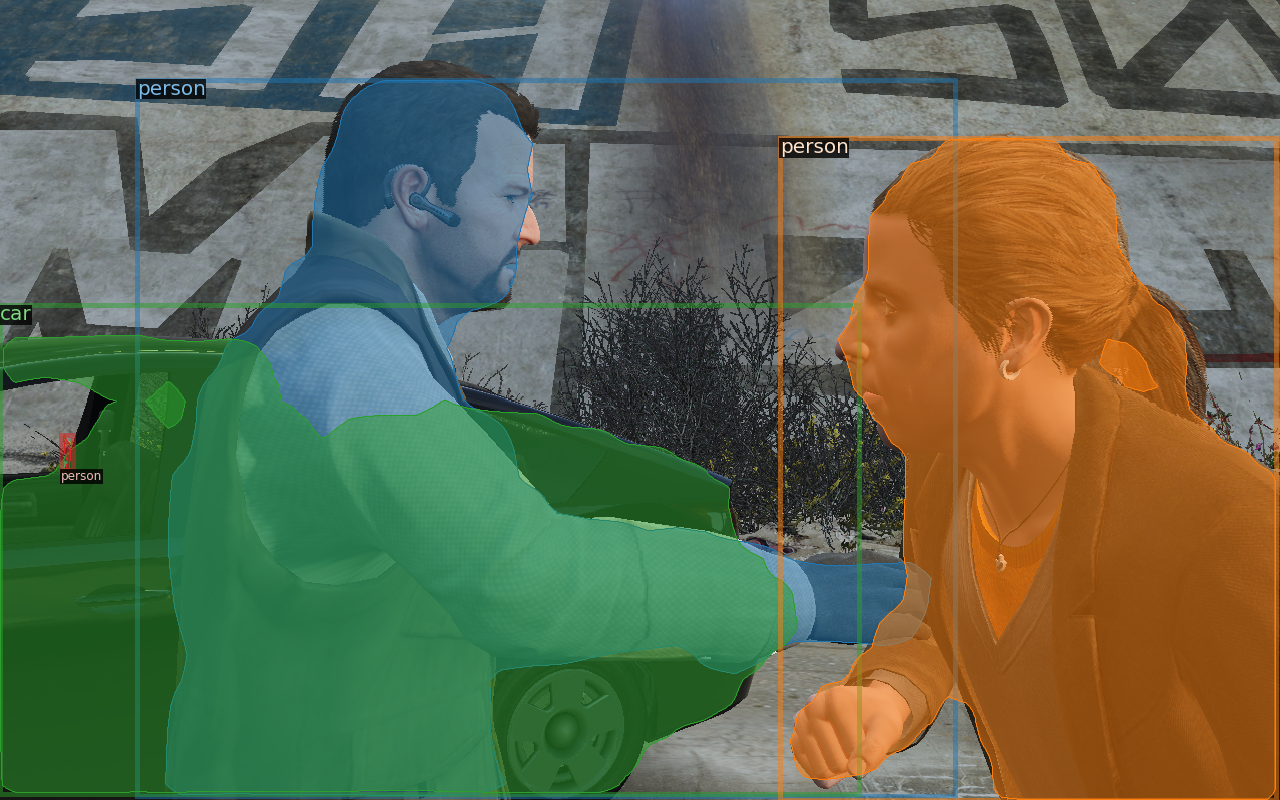
\includegraphics[align=c,width=0.23\linewidth]{fig/sailvos_results/11413_base} &
    %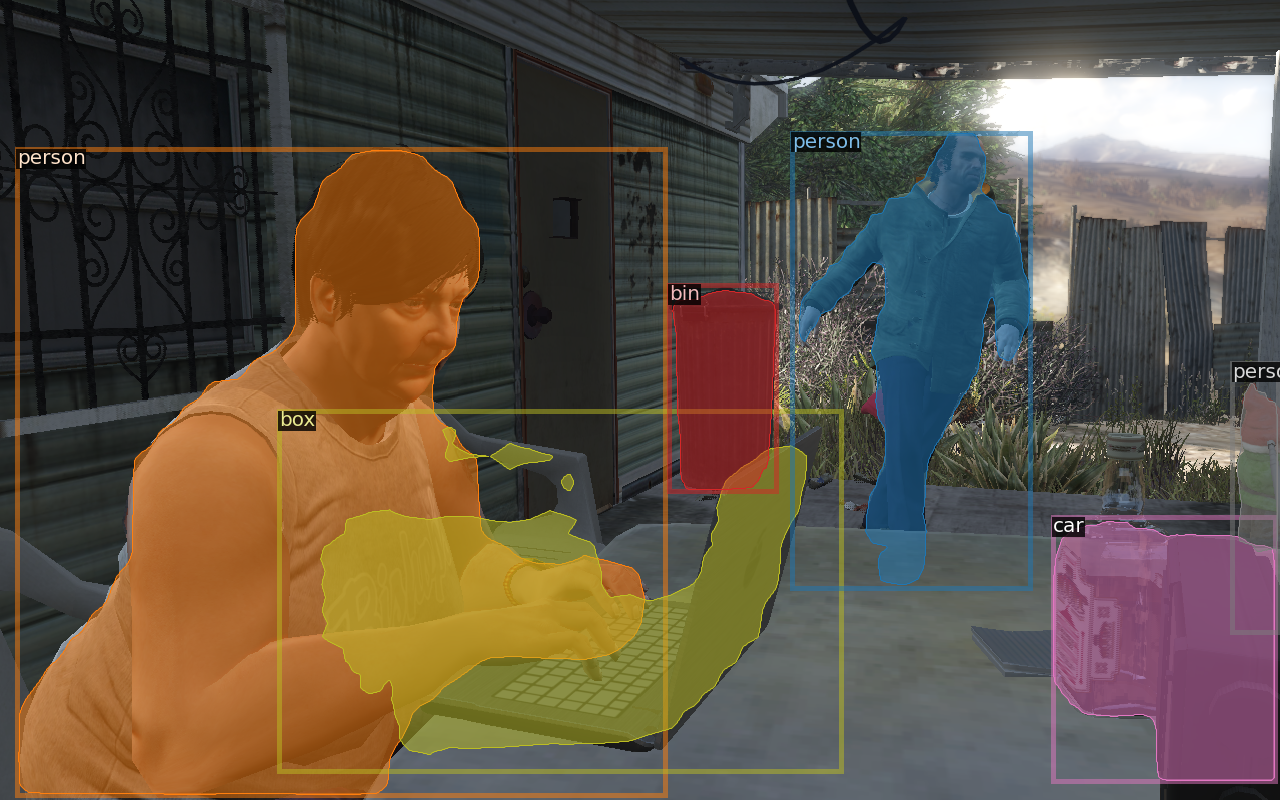
\includegraphics[align=c,width=0.23\linewidth]{fig/sailvos_results/22243_base}
    %\\
    %% Ours
    %Ours &
    %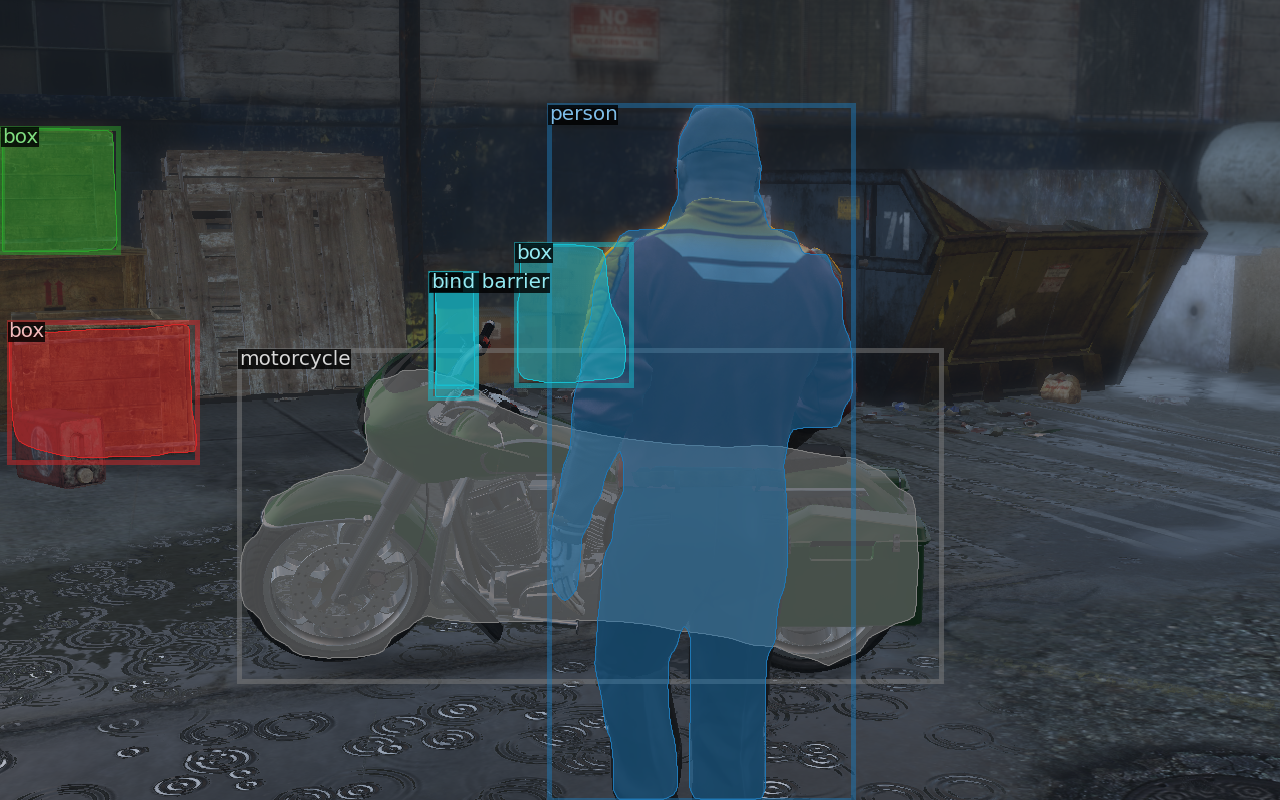
\includegraphics[align=c,width=0.23\linewidth]{fig/sailvos_results/14498_ours} &
    %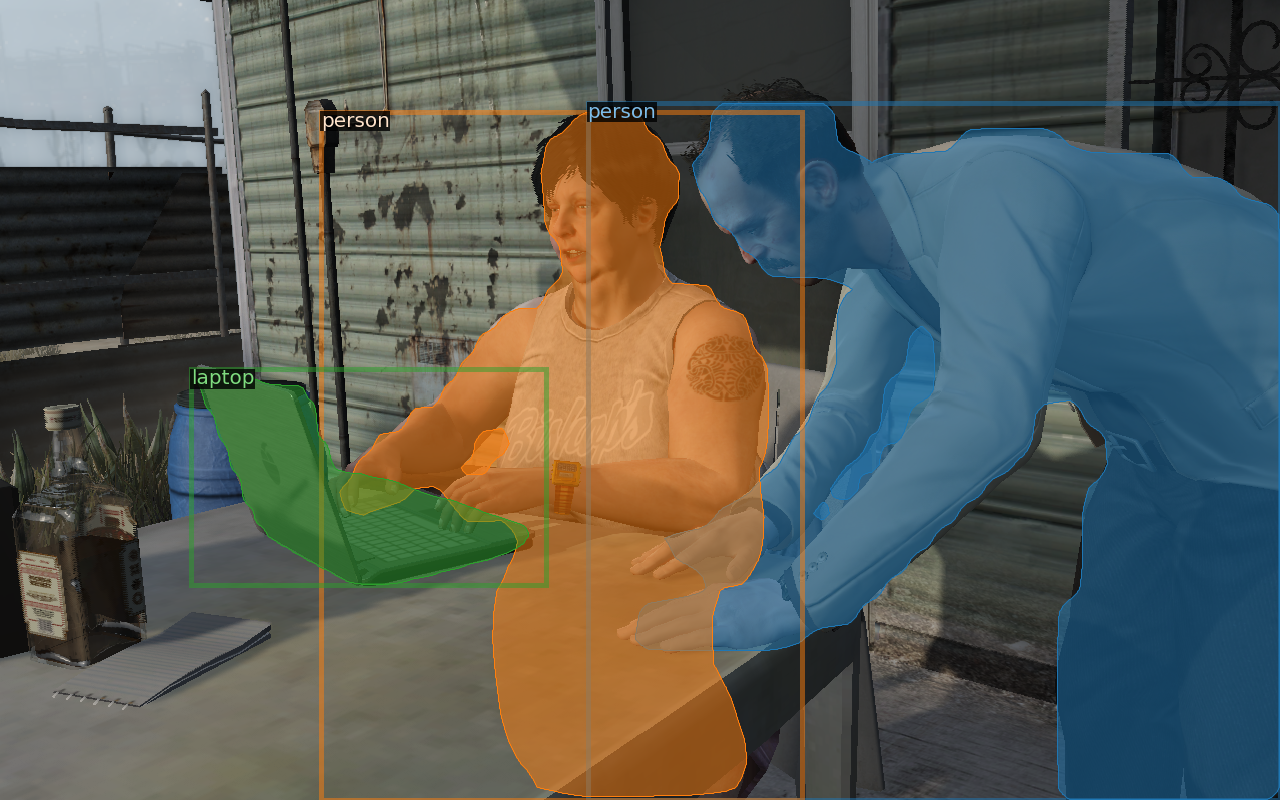
\includegraphics[align=c,width=0.23\linewidth]{fig/sailvos_results/21781_ours} &
    %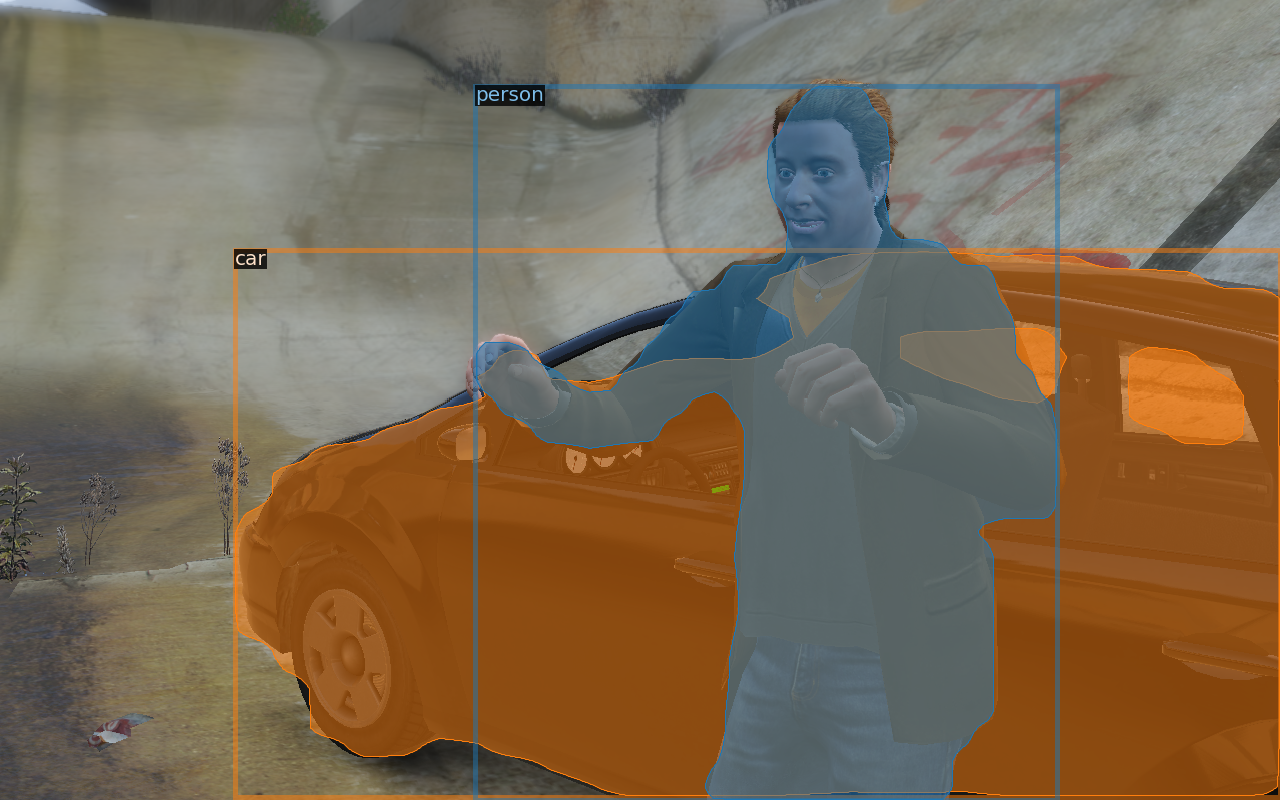
\includegraphics[align=c,width=0.23\linewidth]{fig/sailvos_results/10561_ours} &
    %%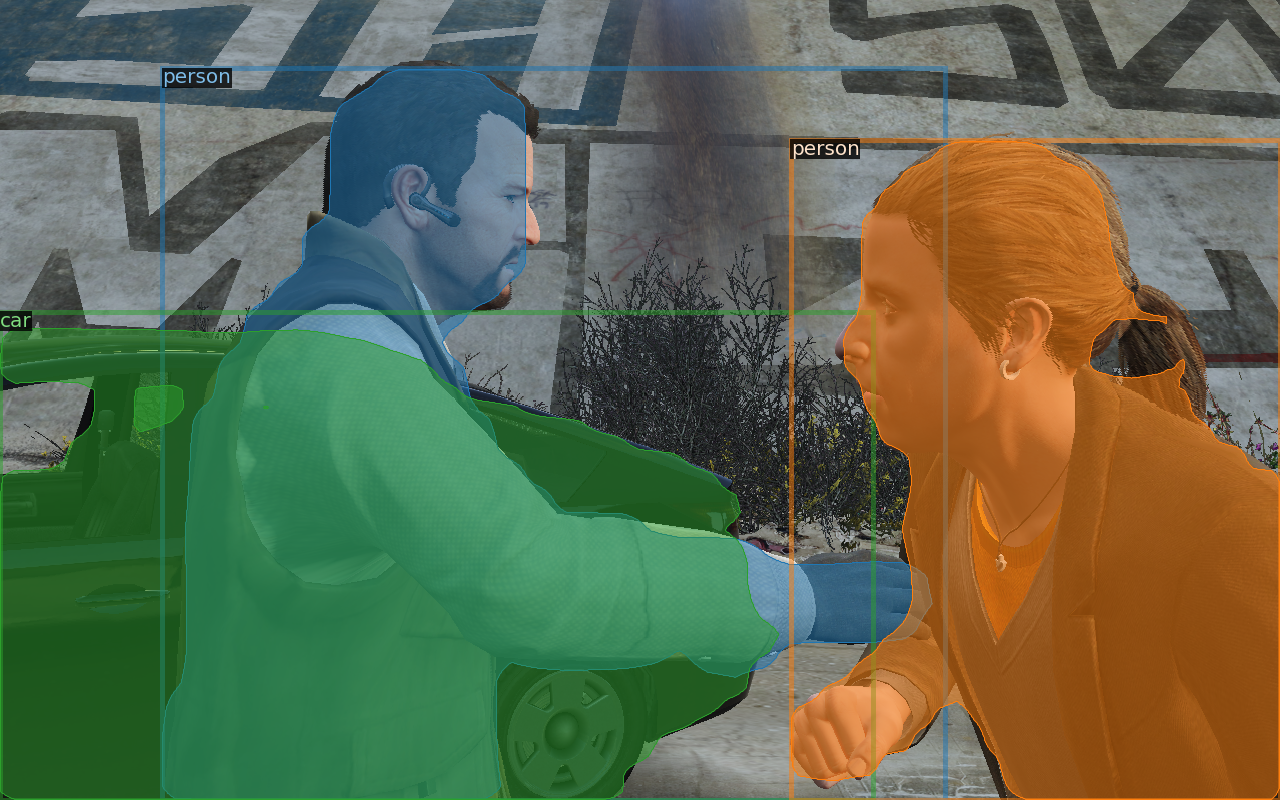
\includegraphics[align=c,width=0.23\linewidth]{fig/sailvos_results/11413_ours} &
    %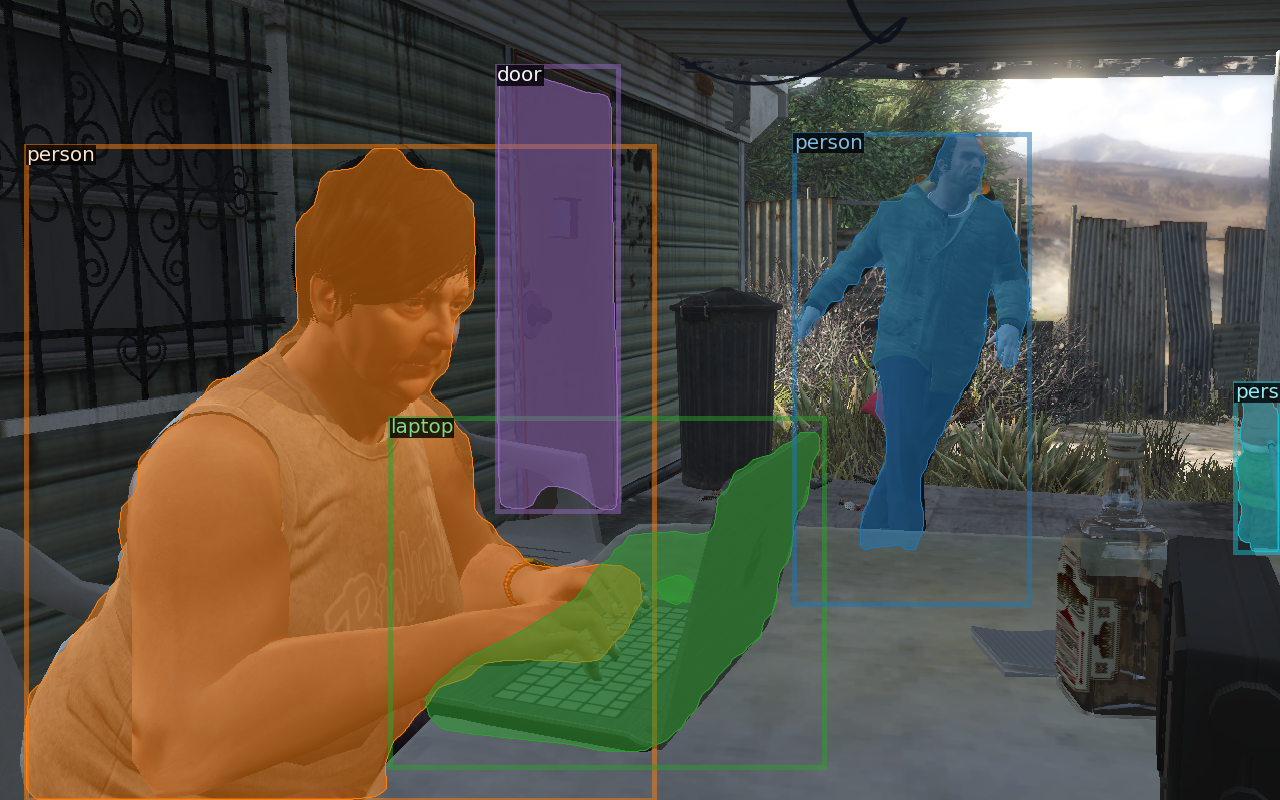
\includegraphics[align=c,width=0.23\linewidth]{fig/sailvos_results/22243_ours}
    %\end{tabular}
    
    %\begin{tabular}{ccc}
    %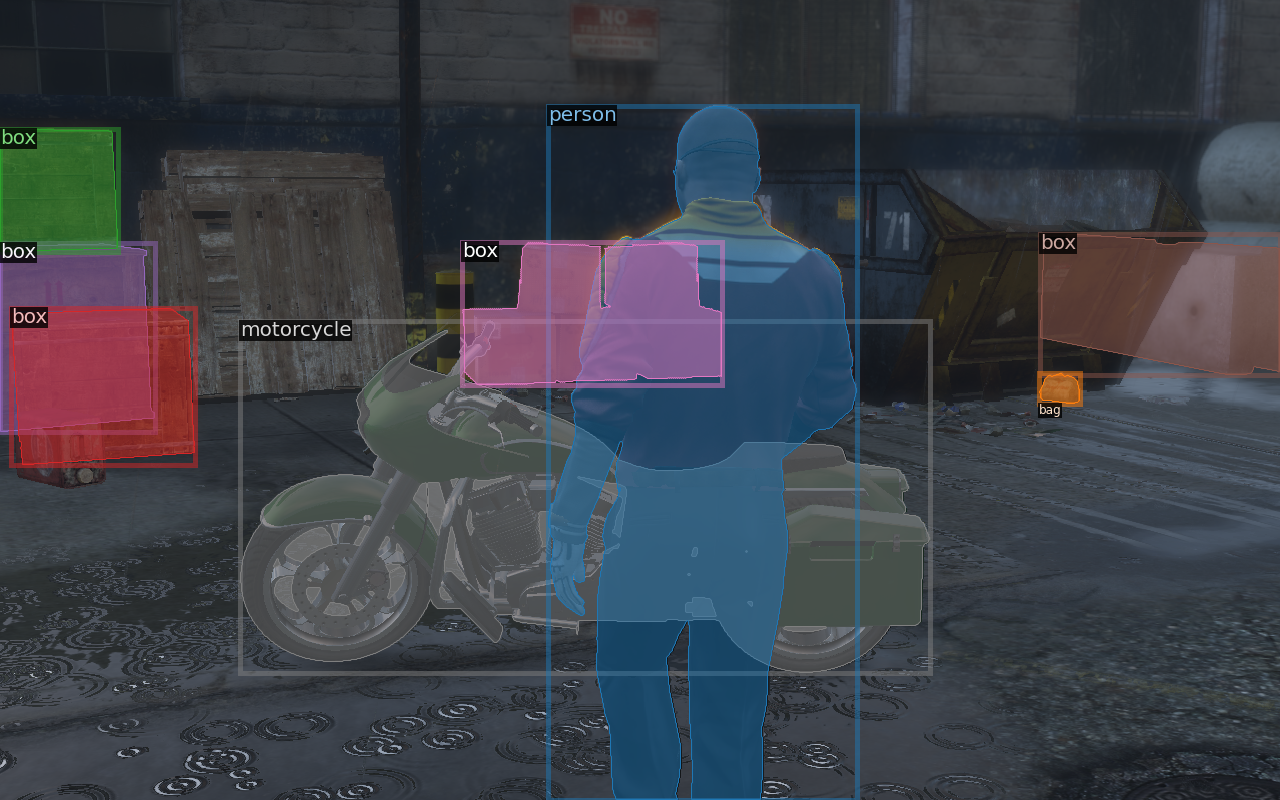
\includegraphics[width=0.31\linewidth]{fig/sailvos_results/14498_gt} & 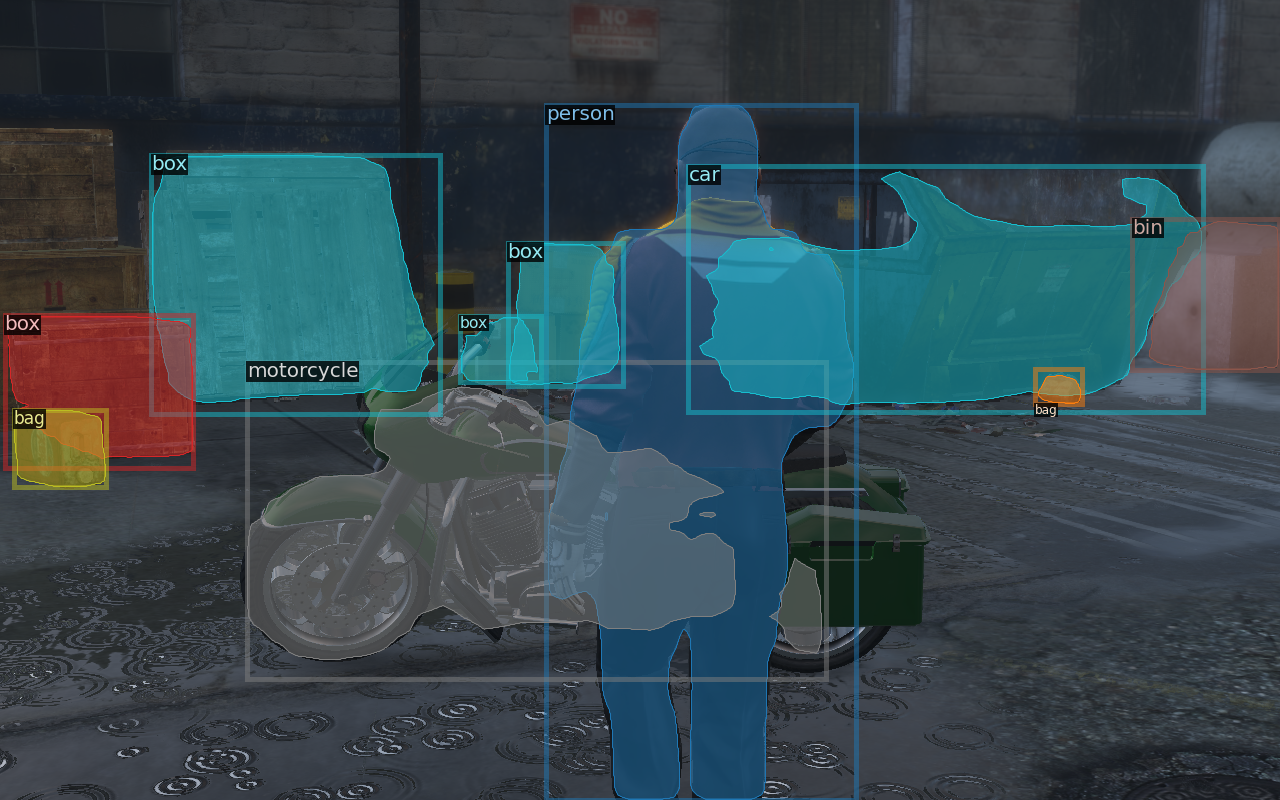
\includegraphics[width=0.31\linewidth]{fig/sailvos_results/14498_base} & 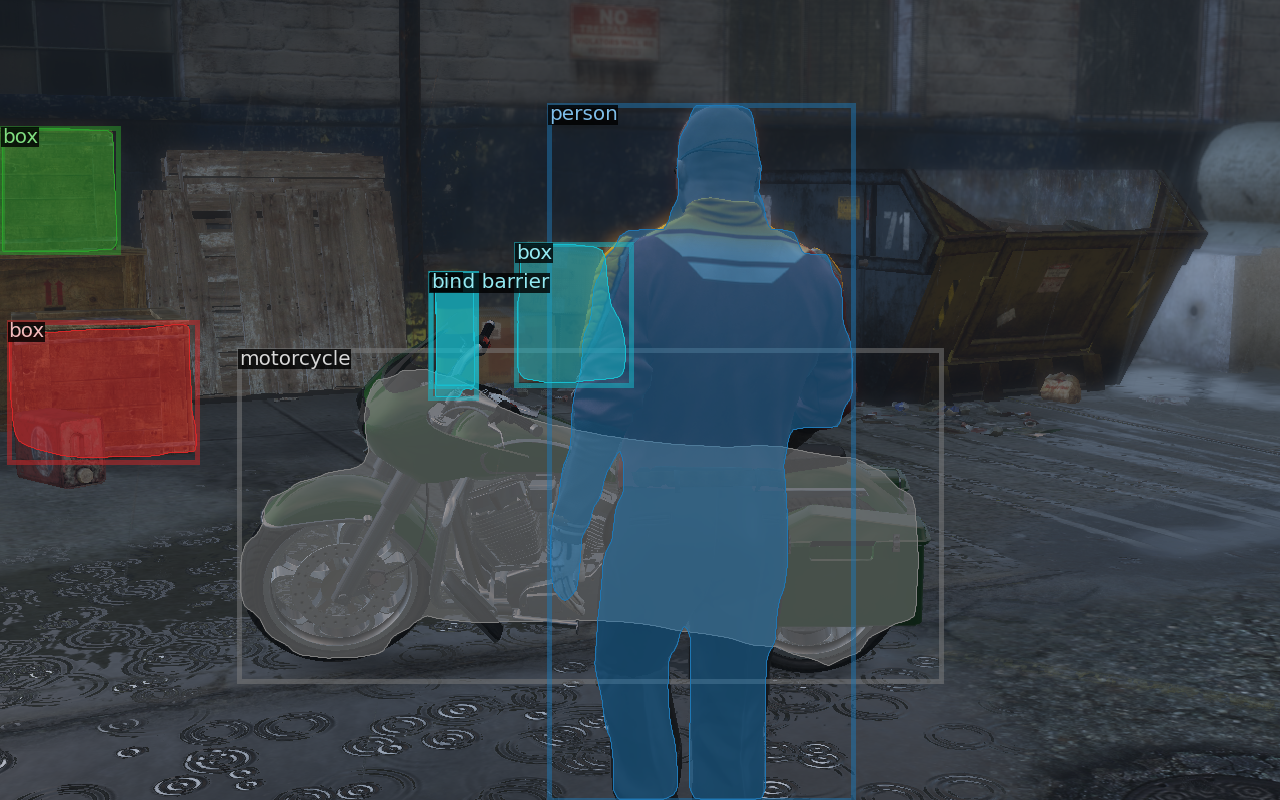
\includegraphics[width=0.31\linewidth]{fig/sailvos_results/14498_ours}\\
    %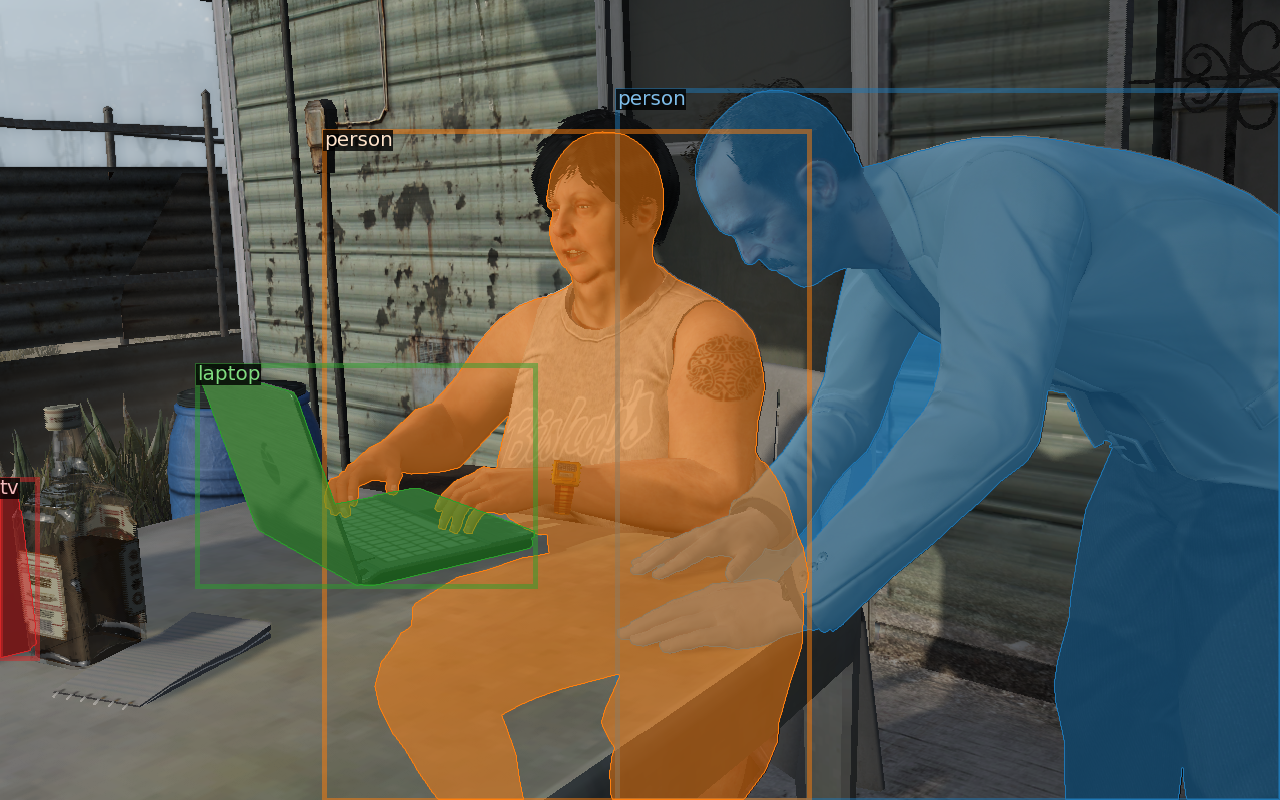
\includegraphics[width=0.31\linewidth]{fig/sailvos_results/21781_gt} &
    %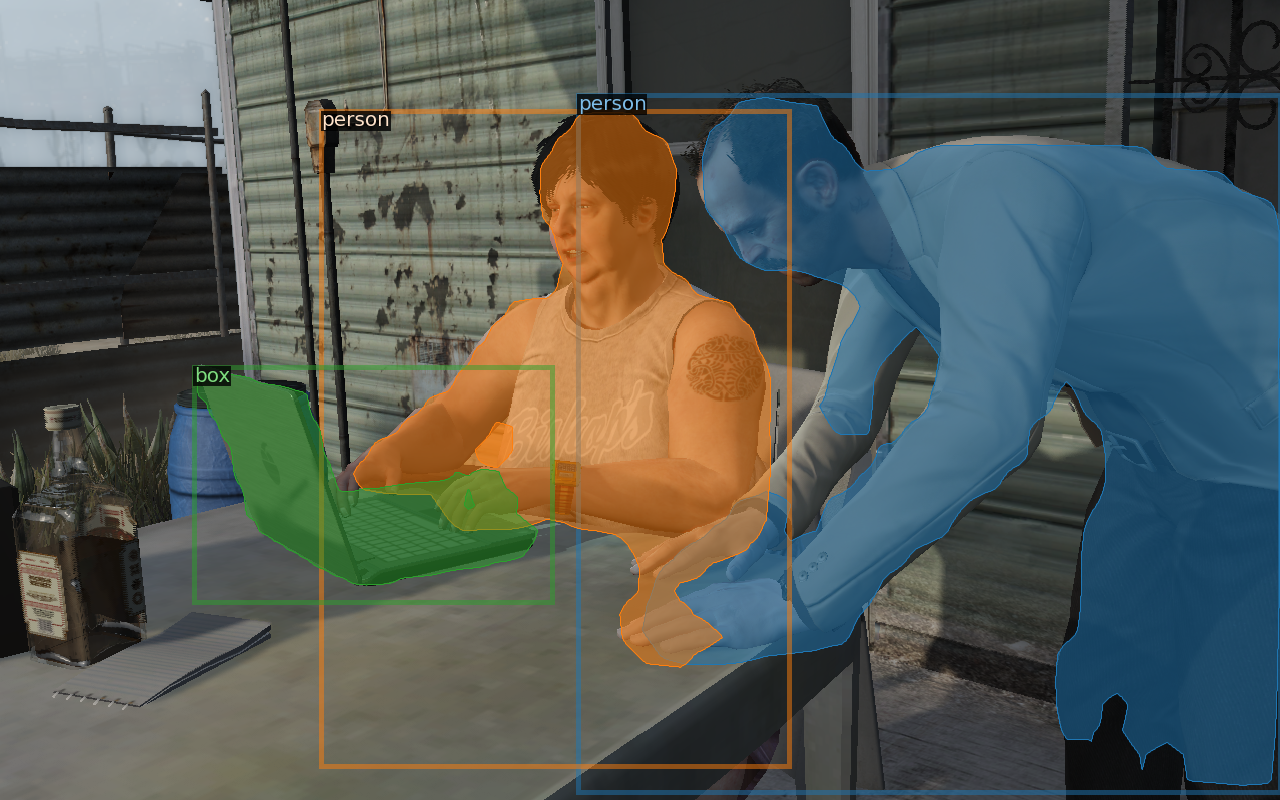
\includegraphics[width=0.31\linewidth]{fig/sailvos_results/21781_base} &
    %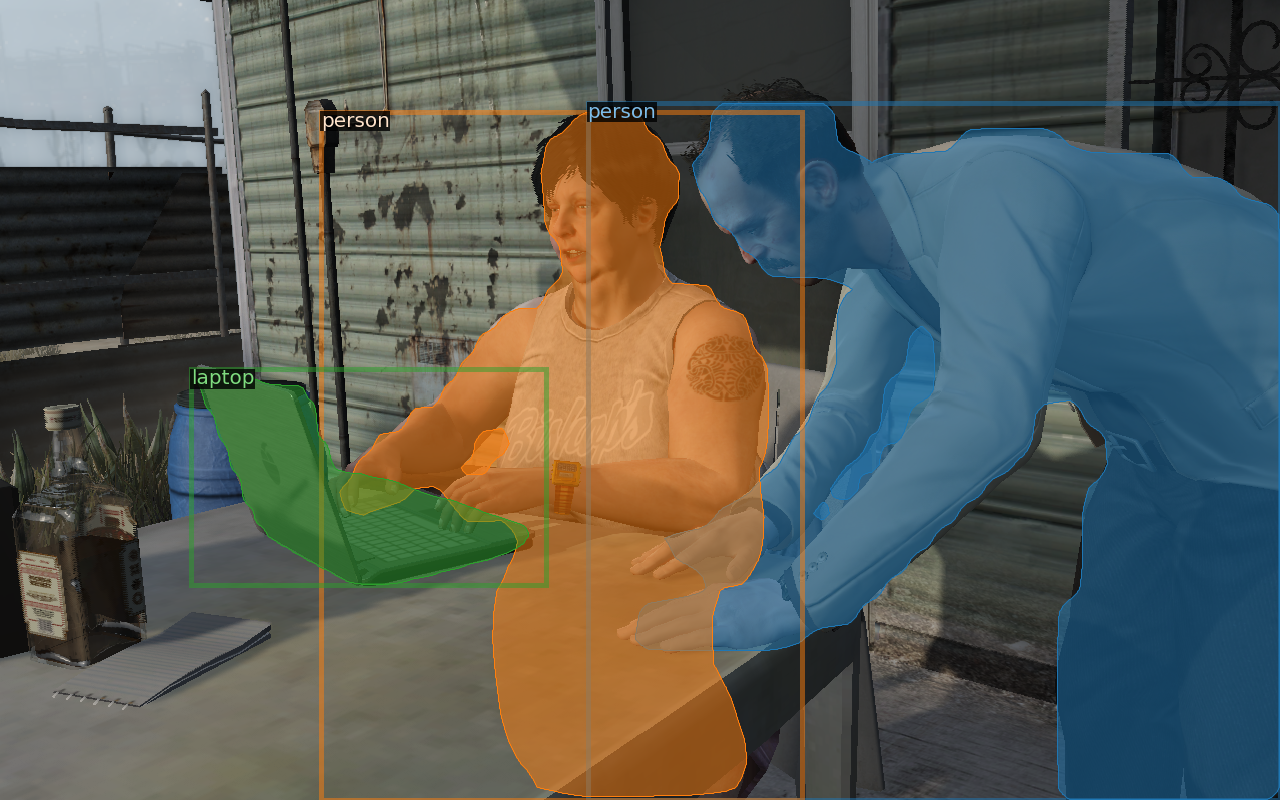
\includegraphics[width=0.31\linewidth]{fig/sailvos_results/21781_ours}\\
    %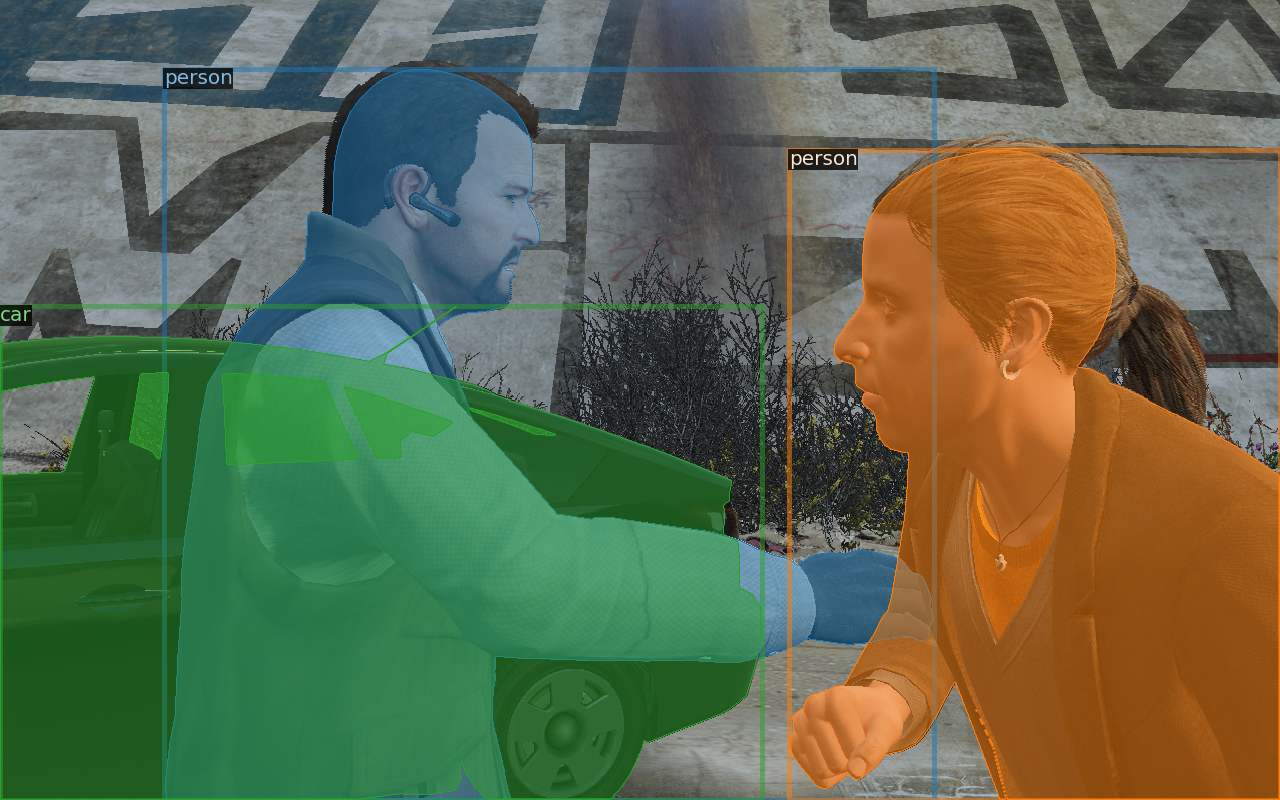
\includegraphics[width=0.31\linewidth]{fig/sailvos_results/11413_gt} & 
    %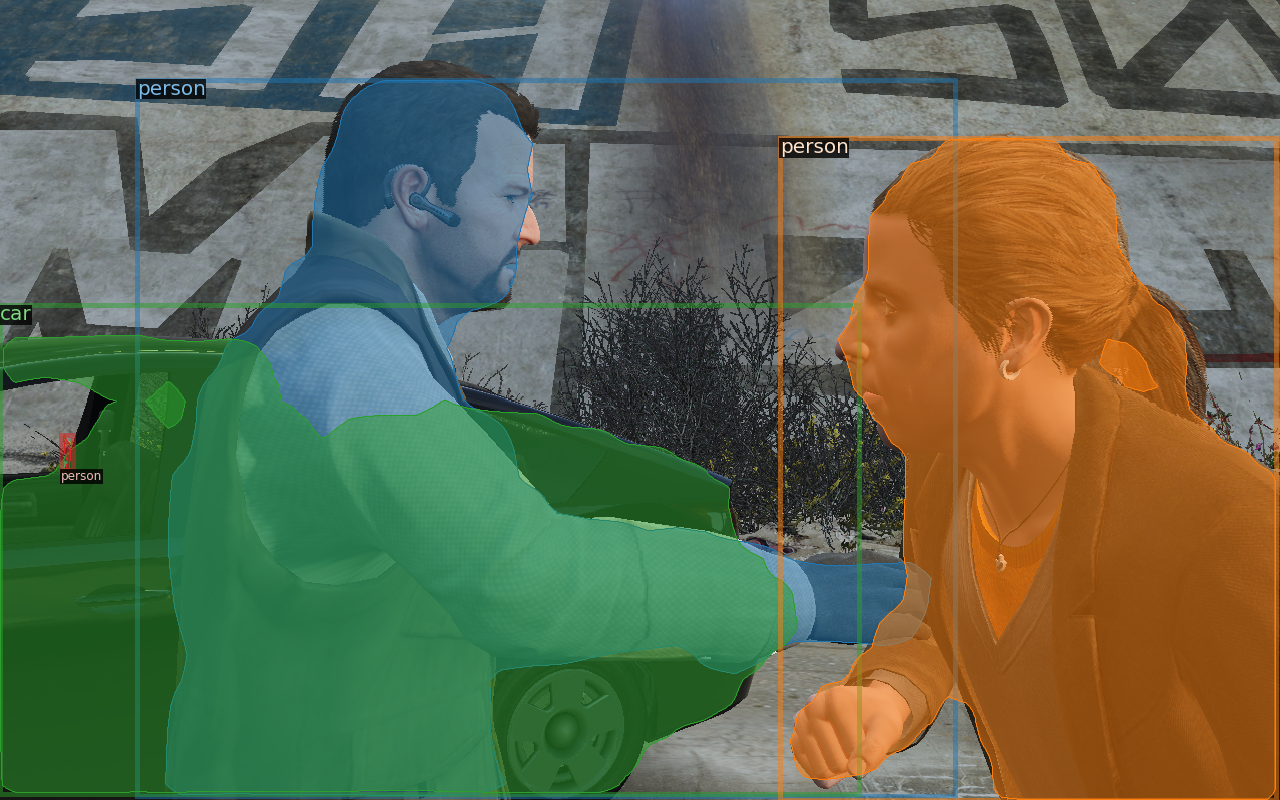
\includegraphics[width=0.31\linewidth]{fig/sailvos_results/11413_base} & 
    %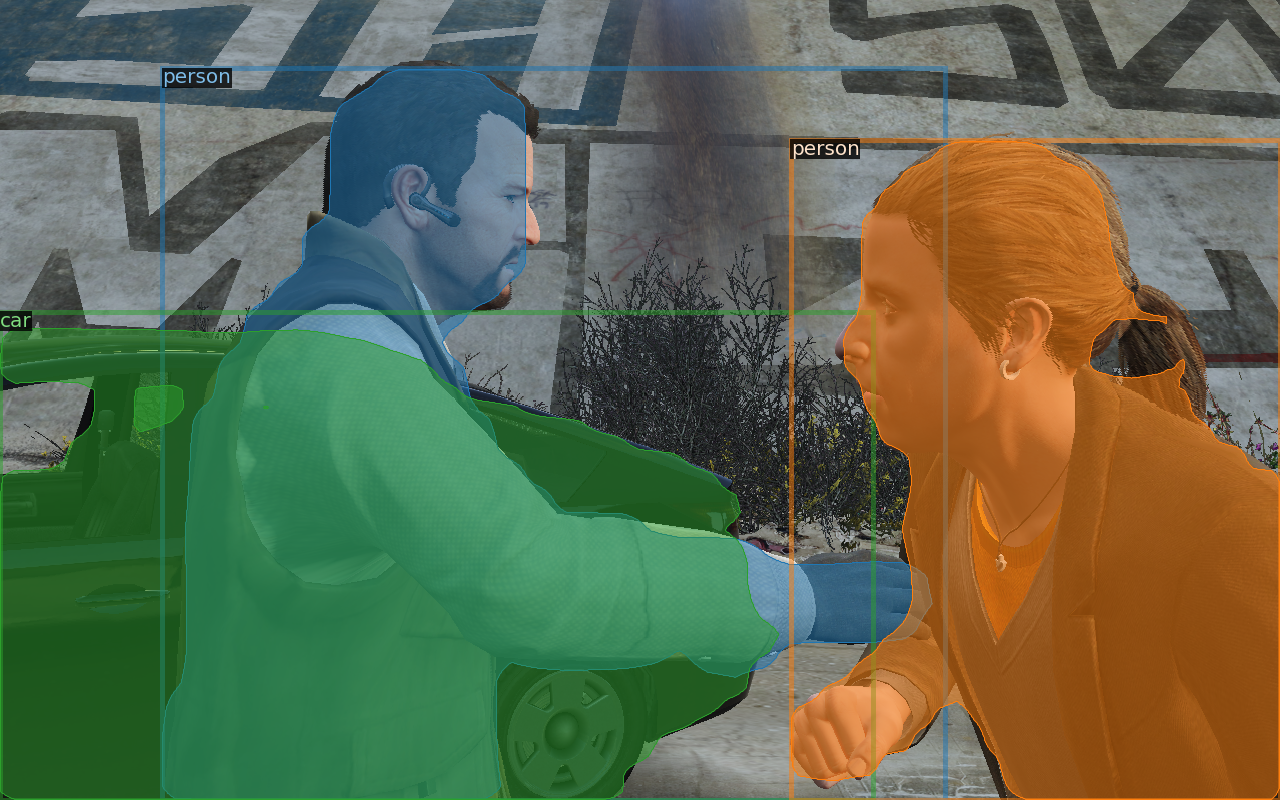
\includegraphics[width=0.31\linewidth]{fig/sailvos_results/11413_ours}\\
    %GT & MaskJoint & Ours
    %\end{tabular}
    
    %\begin{figure*}[t]
    %{
    %\centering
    %\includegraphics[width=0.99\textwidth]{fig/sailvos_results/21781}
    %\includegraphics[width=0.99\textwidth]{fig/sailvos_results/14498}\\
    %}
    %\hspace{2.9cm}Ground-Truth  \hspace{2.8cm} MaskJoint~\cite{hu2019sail}  \hspace{3.2cm} Oursz
    %\caption{Qualitative comparisons with~\cite{hu2019sail} on SAILVOS dataset. 
    %}
    %\label{fig:qual_result}
    %\end{figure*}
    
%!TEX root = ../main.tex
\begin{table*}[t]
\centering
\renewcommand{\arraystretch}{0.95}
\begin{tabular*}{\textwidth}{@{\extracolsep{\fill}}c|ccccccccc}
\specialrule{.15em}{.05em}{.05em}
Row \# & Method &  Occlude & Flow & \# Mask Layers & Cascade & Soft-NMS & Mask Iter. & Box AP & Mask AP\\
\hline\hline
%MaskAmodal~\cite{follmann2019learning} & \xmark & \xmark & 4 & \xmark & \xmark & \xmark & - & 13.0\\ 
%MaskJoint~\cite{hu2019sail} & \xmark & \xmark & 4 & \xmark & \xmark & \xmark & - & 14.1\\
1 & MaskJoint~\cite{hu2019sail} & \xmark&  \xmark & 4 & \xmark & \xmark  & \xmark & - & 14.1\\
2 & Ours & \cmark & \xmark & 4 & \xmark & \xmark  & \xmark & 16.4 & 14.6\\
\hline 
3 & Ours & \cmark & \xmark & 9 &\xmark  & \xmark & \xmark & 16.4  & 15.4\\
4 & Ours & \cmark & \xmark & 10 &\xmark  & \xmark & \xmark &  16.4 & 15.3\\
\hline
5 & Ours & \cmark & \cmark & 9 &\xmark  & \xmark & \xmark &  17.5 & 16.3 \\
\hline 
6 & Ours & \cmark & \cmark & 9 &\cmark  & \xmark & \xmark &  18.6 & 16.7 \\
7 & Ours & \cmark & \cmark & 9 &\cmark  & \cmark & \xmark &   19.6 & 17.3\\
8 & Ours & \cmark & \cmark & 9 &\cmark  & \cmark & \cmark &  \bf 19.6 & \bf 17.6\\
%\cite{hu2019sail} & \xmark & \xmark & - & 13.0 & - & -\\

%\hline
%Ours & \xmark & \xmark &  16.24 & 14.15 & - & - \\
%Ours & \cmark & \cmark &   16.40 & 14.58 & 14.47 & 1.502\\
%\hline
%Ours+6conv. & \xmark & \xmark &  16.26 & 14.90 & - & -\\
%Ours+6conv. & \cmark & \cmark & 16.40  & 15.39 & 14.98 & 2.002\\
%Ours+5conv. & \cmark & \cmark & 16.40  & 15.39 & 14.98 & 2.002\\
%\hline
%Ours+5conv.+flow+soft\_nms & \cmark & \cmark & \bf 17.47 & \bf 16.25 & \bf 15.82 & \bf 2.079\\
\specialrule{.15em}{.05em}{.05em}
\end{tabular*}
\vspace{-0.3cm}
\caption{Ablation study for each of the proposed components on the SAIL-VOS dataset using the class-specific setting.}
\label{tab:abalation}
\vspace{-0.5cm}
\end{table*}





\section{Reprojeciton Results}
We report quantitative results in \ref{tab:sailvos_quan}. The fourth line and the fifth line shows the result of the experiments that study the effect of reprojection. These results are achieved by training 25k iterations with a learning rate of $0.0002$ and a batchsize of $8$. Both of these two experiments outperform the MaskJoint baseline on the second line. However, the best Amodal-net on the third line achieves better result than both of them. The difference in performance is due to the diffrence in training parameters, and the fact that the Amodal-net experiments explored more hyperparameters. The Amodal-net experiment that achieved the highest AP used $9$ mask layers, while the reprojection experiments used $4$. Also, Amodal-net experiments jointly trained modal masks, amodal maks and occluded masks, while the reprojection experiments did not due to computation limitations. The accuracy of the model with or without reprojection can probably get higher if hyperparameters \eg learning rate and batchsize are tuned with more experiments. 



\begin{table*}[t]
%\small
\centering
\setlength{\tabcolsep}{4pt}
\renewcommand{\arraystretch}{0.95}
\begin{tabular*}{\textwidth}{@{\extracolsep{\fill}}c|cccccccc}
\specialrule{.15em}{.05em}{.05em}
 %@{\extracolsep{\fill}}
& \multicolumn{7}{c}{\bf SAIL-VOS class-specific} &  \\
Method & AP &  $\text{AP}_{\text{50}}$ & $\text{AP}_{\text{50}}^{\text{P}}$ & $\text{AP}_{\text{50}}^{\text{H}}$ & $\text{AP}_{\text{50}}^{\text{L}}$ & $\text{AP}_{\text{50}}^{\text{M}}$ & $\text{AP}_{\text{50}}^{\text{S}}$ 

\\
\hline\hline
MaskAmodal~ & 
13.0 & 23.0 & 24.3 & 16.7 & 36.6 & 21.5 & 6.1 & \\% Class-specific

%40.4 & 26.6\\

MaskJoint~\cite{hu2019sail} &
14.1 & 24.8 & 24.3 & 18.9 & 37.8 & 21.5 & 5.7 & \\  % Class-specific

Base model(Amodal-Net) & 
\bf 17.6 & \bf 28.3 &  \bf 28.9 & \bf 20.1 &  \bf 47.1 & \bf 24.8 & \bf 10.6& \\% Class-Agnostic

\hline
 Base model with reprojection & 
 - &  - &   - &  - &   - & - & -& \\ % Class-Agnostic

 Base model without reprojection & 
- & - &  - & - &  - & - & - & \\


\specialrule{.15em}{.05em}{.05em}
\end{tabular*}
\vspace{-0.3cm}
\caption{Quantitative amodal segmentation results for the SAIL-VOS dataset using class-specific and class-agnostic settings.
%\ray{Class-agnostic heavy needs some tunining?}
}
\vspace{-0.45cm}
\label{tab:sailvos_quan}
\end{table*}
 

Comparing the last two rows in \ref{tab:sailvos_quan}, we can see that reprojection performs better in the mask AP metric by $0.1$. However, the difference is not significant, and the training without reprojection preforms better in some other metrics. In general, the two versions achieved similar results as we can see in \ref{fig:ap}. Note that we are discussing the training after 25k iterations in \ref{fig:ap}, \ref{fig:ap_bin}, \ref{fig:ap_box} and \ref{fig:ap_person} not the full 40k iterations. 

If we look at the metrics per class, we can see that training with reprojection performs better for objects that are static \eg box and bin \ref{fig:ap_bin}. But for object that moves \eg person \ref{fig:ap_person}, it performs worse than the training without reprojection. This obeservation matches the fact that reprojection only considers camera movement and not the object movemtn. In other words, reprojection will only align objects assuming they are still. 

If we look at the performance for different object sizes, the two performs similarly in large and medium objects. But interestingly, reprojection achieves better result for small objects, as it achieves $0.2$ AP higher than training without reprojection. This could be due to the fact that there is a higher percentage of static objects that are small compared to medium and large objects. For example, boxes and bins are usually far away in the scene and thus smaller compared to people.

 

[TODO: add qualiatative result here]

\begin{figure*}[t]
\centering
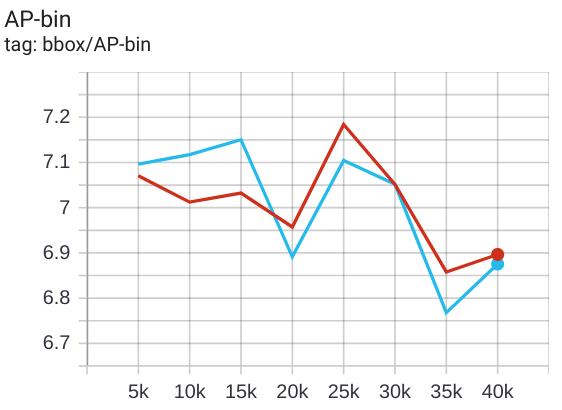
\includegraphics[width=0.6\textwidth]{fig/ap.png}
\vspace{-0.35cm}
\caption{AP on the test dataset during training}
\vspace{-0.4cm}
\label{fig:ap}
\end{figure*}

\begin{figure*}[t]
\centering
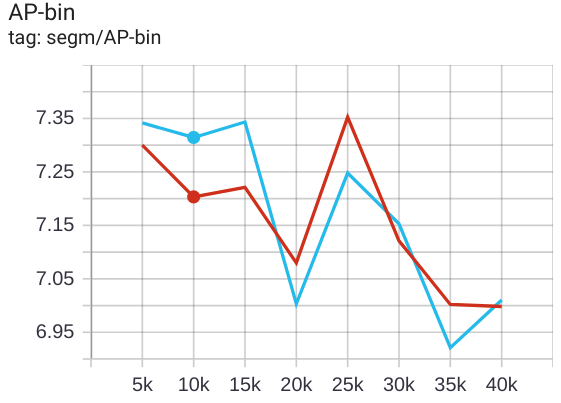
\includegraphics[width=0.6\textwidth]{fig/ap_bin_s.png}
\vspace{-0.35cm}
\caption{AP for object class 'bin' on the test dataset during training}
\vspace{-0.4cm}
\label{fig:ap_bin}
\end{figure*}

\begin{figure*}[t]
\centering
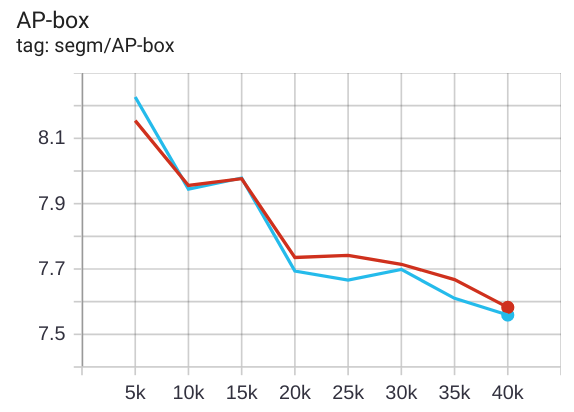
\includegraphics[width=0.6\textwidth]{fig/ap_box_s.png}
\vspace{-0.35cm}
\caption{AP for object class 'box' on the test dataset during training}
\vspace{-0.4cm}
\label{fig:ap_box}
\end{figure*}

\begin{figure*}[t]
\centering
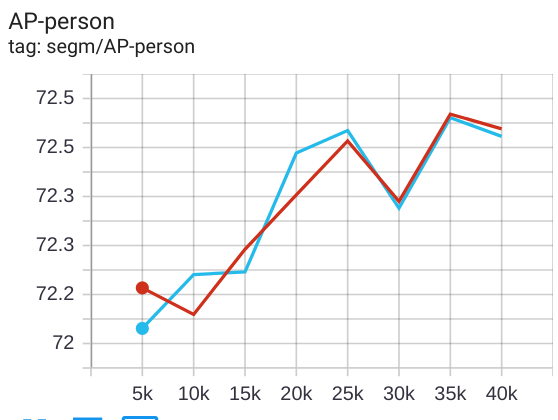
\includegraphics[width=0.6\textwidth]{fig/ap_person_s.png}
\vspace{-0.35cm}
\caption{AP for object class 'person' on the test dataset during training}
\vspace{-0.4cm}
\label{fig:ap_person}
\end{figure*}




\section{Hyperparameter}
The next step we conducted experiments to tune the hyperparameters. In particular, we launched many experiements with different learning rates. As shown in \ref{tab:ablation_reproj}, we experimented with learning rate from $0.02$ to $2\times 10^{-4}$. We can see that learning rate has a big impact on training. In all the runs, there is a decay of learning rate in the last $5000$ and $2500$ iterations by a factor of $0.1$ and $0.1^2$. Since in the start of training, we are loading the pre-trained weights, the experiments with larger learning rates saw a big regression in the start of the training. Some of them never outperformed the baseline due to the initial decline, which is reported in the first row. On the other hand, using a smaller learning rate means that the model will not change much from its initial state, which implies that the gain in performance will also not be too significant. 
%!TEX root = ../main.tex
\begin{table*}[t]
\centering
\renewcommand{\arraystretch}{0.95}
\scalebox{0.9}{
\begin{tabular}{@{\extracolsep{\fill}}c|ccccccccc}
\specialrule{.15em}{.05em}{.05em}
Row \# & Method &  lr & Batchsize &Occlude & Alignment & \# Mask Layers & Amodal feats & Box AP & Mask AP\\
\hline\hline
%MaskAmodal~\cite{follmann2019learning} & \xmark & \xmark & 4 & \xmark & \xmark & \xmark & - & 13.0\\ 
%MaskJoint~\cite{hu2019sail} & \xmark & \xmark & 4 & \xmark & \xmark & \xmark & - & 14.1\\
1 & MaskJoint~\cite{hu2019sail} & - & - & \xmark&  \xmark & 4 & \xmark & - & 14.1\\
2 & Ours & - & 16 & \cmark & Flow & 9 &\cmark  &  \bf 19.6 & \bf 17.6\\
\hline
3 & Ours & 2e-2 & 8 & \cmark & Reproj & 4 &\cmark  &  12.99 & 12.22 \\
4 & Ours & 2e-3 & 8 & \cmark & Reproj & 4 &\cmark  &  16.55 & 14.67 \\
5 & Ours & 6e-3 & 8 & \cmark & Reproj & 4 &\cmark  &   14.93 &  13.35\\
6 & Ours & 2e-4 & 8 & \cmark & Reproj & 4 &\cmark  &   16.86 & \bf 15.04\\
7 & Ours & 2e-4 & 8 & \cmark & \xmark & 4 &\cmark  &  \bf 16.91 & 15.01\\
%\cite{hu2019sail} & \xmark & \xmark & - & 13.0 & - & -\\

%\hline
%Ours & \xmark & \xmark &  16.24 & 14.15 & - & - \\
%Ours & \cmark & \cmark &   16.40 & 14.58 & 14.47 & 1.502\\
%\hline
%Ours+6conv. & \xmark & \xmark &  16.26 & 14.90 & - & -\\
%Ours+6conv. & \cmark & \cmark & 16.40  & 15.39 & 14.98 & 2.002\\
%Ours+5conv. & \cmark & \cmark & 16.40  & 15.39 & 14.98 & 2.002\\
%\hline
%Ours+5conv.+flow+soft\_nms & \cmark & \cmark & \bf 17.47 & \bf 16.25 & \bf 15.82 & \bf 2.079\\
\specialrule{.15em}{.05em}{.05em}
\end{tabular}}
\vspace{-0.3cm}
\caption{Ablation study for hyperparameters in experiments on reprojection. 'Amodal feats' column refers to three features added in Amodal-net: cascade, Soft-NMS and Mask-Iter}
\label{tab:ablation_reproj}
\vspace{-0.5cm}
\end{table*}
    
    
    

 